% Options for packages loaded elsewhere
\PassOptionsToPackage{unicode}{hyperref}
\PassOptionsToPackage{hyphens}{url}
%
\documentclass[
  ignorenonframetext,
]{beamer}
\usepackage{pgfpages}
\setbeamertemplate{caption}[numbered]
\setbeamertemplate{caption label separator}{: }
\setbeamercolor{caption name}{fg=normal text.fg}
\beamertemplatenavigationsymbolsempty
% Prevent slide breaks in the middle of a paragraph
\widowpenalties 1 10000
\raggedbottom
\setbeamertemplate{part page}{
  \centering
  \begin{beamercolorbox}[sep=16pt,center]{part title}
    \usebeamerfont{part title}\insertpart\par
  \end{beamercolorbox}
}
\setbeamertemplate{section page}{
  \centering
  \begin{beamercolorbox}[sep=12pt,center]{part title}
    \usebeamerfont{section title}\insertsection\par
  \end{beamercolorbox}
}
\setbeamertemplate{subsection page}{
  \centering
  \begin{beamercolorbox}[sep=8pt,center]{part title}
    \usebeamerfont{subsection title}\insertsubsection\par
  \end{beamercolorbox}
}
\AtBeginPart{
  \frame{\partpage}
}
\AtBeginSection{
  \ifbibliography
  \else
    \frame{\sectionpage}
  \fi
}
\AtBeginSubsection{
  \frame{\subsectionpage}
}
\usepackage{amsmath,amssymb}
\usepackage{iftex}
\ifPDFTeX
  \usepackage[T1]{fontenc}
  \usepackage[utf8]{inputenc}
  \usepackage{textcomp} % provide euro and other symbols
\else % if luatex or xetex
  \usepackage{unicode-math} % this also loads fontspec
  \defaultfontfeatures{Scale=MatchLowercase}
  \defaultfontfeatures[\rmfamily]{Ligatures=TeX,Scale=1}
\fi
\usepackage{lmodern}
\usetheme[]{Lumen}
\ifPDFTeX\else
  % xetex/luatex font selection
\fi
% Use upquote if available, for straight quotes in verbatim environments
\IfFileExists{upquote.sty}{\usepackage{upquote}}{}
\IfFileExists{microtype.sty}{% use microtype if available
  \usepackage[]{microtype}
  \UseMicrotypeSet[protrusion]{basicmath} % disable protrusion for tt fonts
}{}
\makeatletter
\@ifundefined{KOMAClassName}{% if non-KOMA class
  \IfFileExists{parskip.sty}{%
    \usepackage{parskip}
  }{% else
    \setlength{\parindent}{0pt}
    \setlength{\parskip}{6pt plus 2pt minus 1pt}}
}{% if KOMA class
  \KOMAoptions{parskip=half}}
\makeatother
\usepackage{xcolor}
\newif\ifbibliography
\usepackage{color}
\usepackage{fancyvrb}
\newcommand{\VerbBar}{|}
\newcommand{\VERB}{\Verb[commandchars=\\\{\}]}
\DefineVerbatimEnvironment{Highlighting}{Verbatim}{commandchars=\\\{\}}
% Add ',fontsize=\small' for more characters per line
\usepackage{framed}
\definecolor{shadecolor}{RGB}{248,248,248}
\newenvironment{Shaded}{\begin{snugshade}}{\end{snugshade}}
\newcommand{\AlertTok}[1]{\textcolor[rgb]{0.94,0.16,0.16}{#1}}
\newcommand{\AnnotationTok}[1]{\textcolor[rgb]{0.56,0.35,0.01}{\textbf{\textit{#1}}}}
\newcommand{\AttributeTok}[1]{\textcolor[rgb]{0.13,0.29,0.53}{#1}}
\newcommand{\BaseNTok}[1]{\textcolor[rgb]{0.00,0.00,0.81}{#1}}
\newcommand{\BuiltInTok}[1]{#1}
\newcommand{\CharTok}[1]{\textcolor[rgb]{0.31,0.60,0.02}{#1}}
\newcommand{\CommentTok}[1]{\textcolor[rgb]{0.56,0.35,0.01}{\textit{#1}}}
\newcommand{\CommentVarTok}[1]{\textcolor[rgb]{0.56,0.35,0.01}{\textbf{\textit{#1}}}}
\newcommand{\ConstantTok}[1]{\textcolor[rgb]{0.56,0.35,0.01}{#1}}
\newcommand{\ControlFlowTok}[1]{\textcolor[rgb]{0.13,0.29,0.53}{\textbf{#1}}}
\newcommand{\DataTypeTok}[1]{\textcolor[rgb]{0.13,0.29,0.53}{#1}}
\newcommand{\DecValTok}[1]{\textcolor[rgb]{0.00,0.00,0.81}{#1}}
\newcommand{\DocumentationTok}[1]{\textcolor[rgb]{0.56,0.35,0.01}{\textbf{\textit{#1}}}}
\newcommand{\ErrorTok}[1]{\textcolor[rgb]{0.64,0.00,0.00}{\textbf{#1}}}
\newcommand{\ExtensionTok}[1]{#1}
\newcommand{\FloatTok}[1]{\textcolor[rgb]{0.00,0.00,0.81}{#1}}
\newcommand{\FunctionTok}[1]{\textcolor[rgb]{0.13,0.29,0.53}{\textbf{#1}}}
\newcommand{\ImportTok}[1]{#1}
\newcommand{\InformationTok}[1]{\textcolor[rgb]{0.56,0.35,0.01}{\textbf{\textit{#1}}}}
\newcommand{\KeywordTok}[1]{\textcolor[rgb]{0.13,0.29,0.53}{\textbf{#1}}}
\newcommand{\NormalTok}[1]{#1}
\newcommand{\OperatorTok}[1]{\textcolor[rgb]{0.81,0.36,0.00}{\textbf{#1}}}
\newcommand{\OtherTok}[1]{\textcolor[rgb]{0.56,0.35,0.01}{#1}}
\newcommand{\PreprocessorTok}[1]{\textcolor[rgb]{0.56,0.35,0.01}{\textit{#1}}}
\newcommand{\RegionMarkerTok}[1]{#1}
\newcommand{\SpecialCharTok}[1]{\textcolor[rgb]{0.81,0.36,0.00}{\textbf{#1}}}
\newcommand{\SpecialStringTok}[1]{\textcolor[rgb]{0.31,0.60,0.02}{#1}}
\newcommand{\StringTok}[1]{\textcolor[rgb]{0.31,0.60,0.02}{#1}}
\newcommand{\VariableTok}[1]{\textcolor[rgb]{0.00,0.00,0.00}{#1}}
\newcommand{\VerbatimStringTok}[1]{\textcolor[rgb]{0.31,0.60,0.02}{#1}}
\newcommand{\WarningTok}[1]{\textcolor[rgb]{0.56,0.35,0.01}{\textbf{\textit{#1}}}}
\usepackage{longtable,booktabs,array}
\usepackage{calc} % for calculating minipage widths
\usepackage{caption}
% Make caption package work with longtable
\makeatletter
\def\fnum@table{\tablename~\thetable}
\makeatother
\usepackage{graphicx}
\makeatletter
\def\maxwidth{\ifdim\Gin@nat@width>\linewidth\linewidth\else\Gin@nat@width\fi}
\def\maxheight{\ifdim\Gin@nat@height>\textheight\textheight\else\Gin@nat@height\fi}
\makeatother
% Scale images if necessary, so that they will not overflow the page
% margins by default, and it is still possible to overwrite the defaults
% using explicit options in \includegraphics[width, height, ...]{}
\setkeys{Gin}{width=\maxwidth,height=\maxheight,keepaspectratio}
% Set default figure placement to htbp
\makeatletter
\def\fps@figure{htbp}
\makeatother
\setlength{\emergencystretch}{3em} % prevent overfull lines
\providecommand{\tightlist}{%
  \setlength{\itemsep}{0pt}\setlength{\parskip}{0pt}}
\setcounter{secnumdepth}{-\maxdimen} % remove section numbering
\ifLuaTeX
  \usepackage{selnolig}  % disable illegal ligatures
\fi
\IfFileExists{bookmark.sty}{\usepackage{bookmark}}{\usepackage{hyperref}}
\IfFileExists{xurl.sty}{\usepackage{xurl}}{} % add URL line breaks if available
\urlstyle{same}
\hypersetup{
  pdftitle={Introduccion a R},
  pdfauthor={Emilio Aguilar Cubilla},
  hidelinks,
  pdfcreator={LaTeX via pandoc}}

\title{Introduccion a R}
\subtitle{Transformando Datos en Historias}
\author{Emilio Aguilar Cubilla}
\date{Marzo, 2024}

\begin{document}
\frame{\titlepage}

\begin{frame}{Quien cuenta historias, domina el mundo - Proverbio Hopi}
\protect\hypertarget{quien-cuenta-historias-domina-el-mundo---proverbio-hopi}{}
\end{frame}

\begin{frame}{Que es R?}
\protect\hypertarget{que-es-r}{}
R es un lenguaje de programación y un entorno de software diseñado
específicamente para estadísticas y análisis de datos. Fue desarrollado
por Ross Ihaka y Robert Gentleman en la Universidad de Auckland, Nueva
Zelanda, en la década de 1990. Desde entonces, R se ha convertido en uno
de los lenguajes más populares en el ámbito de la estadística y la
ciencia de datos

\begin{block}{Características Clave}
\protect\hypertarget{caracteruxedsticas-clave}{}
\begin{enumerate}
\item
  \textbf{Estadísticas y Análisis de Datos:} R es potente para realizar
  análisis estadísticos y exploración de datos, se pueden realizar
  tareas como regresión, análisis de varianza, machine learning, y más.
\item
  \textbf{Gráficos:} R tiene excelentes capacidades para la
  visualización de datos. Puedes crear una variedad de gráficos de alta
  calidad para explorar y comunicar patrones en los datos.
\item
  \textbf{Comunidad y Paquetes:} R tiene una comunidad activa de
  usuarios y desarrolladores. Además, cuenta con un extenso sistema de
  paquetes que amplían sus capacidades.
\item
  \textbf{Investigación Académica y Empresarial:} R se utiliza en
  entornos académicos, de investigación y empresariales
\item
  \textbf{Integración con Otros Lenguajes y Herramientas:} R se puede
  integrar con otros lenguajes de programación como C, C++, y Python.
\end{enumerate}
\end{block}
\end{frame}

\begin{frame}[fragile]{Que es GIT?}
\protect\hypertarget{que-es-git}{}
\textbf{Git} es un sistema de control de versiones distribuido
ampliamente utilizado. Fue creado por Linus Torvalds en 2005 y se ha
convertido en una herramienta esencial para el desarrollo de software
colaborativo.

\begin{block}{Beneficios de Git:}
\protect\hypertarget{beneficios-de-git}{}
\begin{enumerate}
\item
  \textbf{Trabajo Colaborativo:} Git permite a varios desarrolladores
  trabajar en un proyecto simultáneamente sin temor a conflictos. Cada
  desarrollador puede trabajar en su propia rama y fusionar los cambios
  de manera eficiente.
\item
  \textbf{Historial y Auditoría:} El historial completo de cambios en un
  proyecto proporciona una trazabilidad clara y facilita la
  identificación de errores o problemas.
\item
  \textbf{Ramificación:} La capacidad de crear ramas fácilmente facilita
  el desarrollo de nuevas características y la corrección de errores sin
  afectar la rama principal del proyecto.
\item
  \textbf{Flexibilidad:} Git es flexible y se adapta a diversos flujos
  de trabajo, pequeños o grandes
\item
  \textbf{Respaldo y Recuperación:} La distribución y duplicación de
  repositorios proporciona una forma robusta de respaldar y recuperar
  proyectos en caso de fallos.
\end{enumerate}
\end{block}

\begin{block}{Crear usuario en GIT}
\protect\hypertarget{crear-usuario-en-git}{}
\begin{itemize}
\tightlist
\item
  Ir a \url{https://github.com/signup?source=login}
\item
  Crear nuevo usuario
\item
  \textbf{! Crea un usuario facil de escribir y al mismo tiempo que se
  vea profesional}
\item
  GIT tambien es un buen portafolio profesional
\end{itemize}
\end{block}

\begin{block}{Instalacion de R \& GIT}
\protect\hypertarget{instalacion-de-r-git}{}
\begin{block}{Windows:}
\protect\hypertarget{windows}{}
\begin{block}{1. R:}
\protect\hypertarget{r}{}
\begin{itemize}
\tightlist
\item
  Descarga R desde el sitio oficial:
  \url{https://cran.r-project.org/mirrors.html}
\item
  Ejecuta el instalador descargado y sigue las instrucciones.
\end{itemize}
\end{block}

\begin{block}{2. Rtools (opcional pero recomendado para instalar
paquetes adicionales):}
\protect\hypertarget{rtools-opcional-pero-recomendado-para-instalar-paquetes-adicionales}{}
\begin{itemize}
\tightlist
\item
  Descarga Rtools desde
  \url{https://cran.r-project.org/bin/windows/Rtools/}
\item
  Ejecuta el instalador y sigue las instrucciones.
\end{itemize}
\end{block}

\begin{block}{3. Git:}
\protect\hypertarget{git}{}
\begin{itemize}
\tightlist
\item
  Descarga Git desde \url{https://git-scm.com/download/win}
\item
  Ejecuta el instalador descargado y sigue las instrucciones.
\end{itemize}
\end{block}
\end{block}
\end{block}

\begin{block}{Instalacion de R \& GIT}
\protect\hypertarget{instalacion-de-r-git-1}{}
\begin{block}{macOS:}
\protect\hypertarget{macos}{}
\begin{block}{1. R:}
\protect\hypertarget{r-1}{}
\begin{itemize}
\tightlist
\item
  Puedes instalar R usando Homebrew con el siguiente comando en la
  terminal: \texttt{bash\ \ \ \ \ \ brew\ install\ r}
\end{itemize}
\end{block}

\begin{block}{2. Git:}
\protect\hypertarget{git-1}{}
\begin{itemize}
\tightlist
\item
  Puedes instalar Git usando Homebrew con el siguiente comando en la
  terminal: \texttt{bash\ \ \ \ \ \ brew\ install\ git}
\end{itemize}
\end{block}
\end{block}
\end{block}

\begin{block}{Patalla de R}
\protect\hypertarget{patalla-de-r}{}
\begin{figure}
\hypertarget{id}{%
\centering
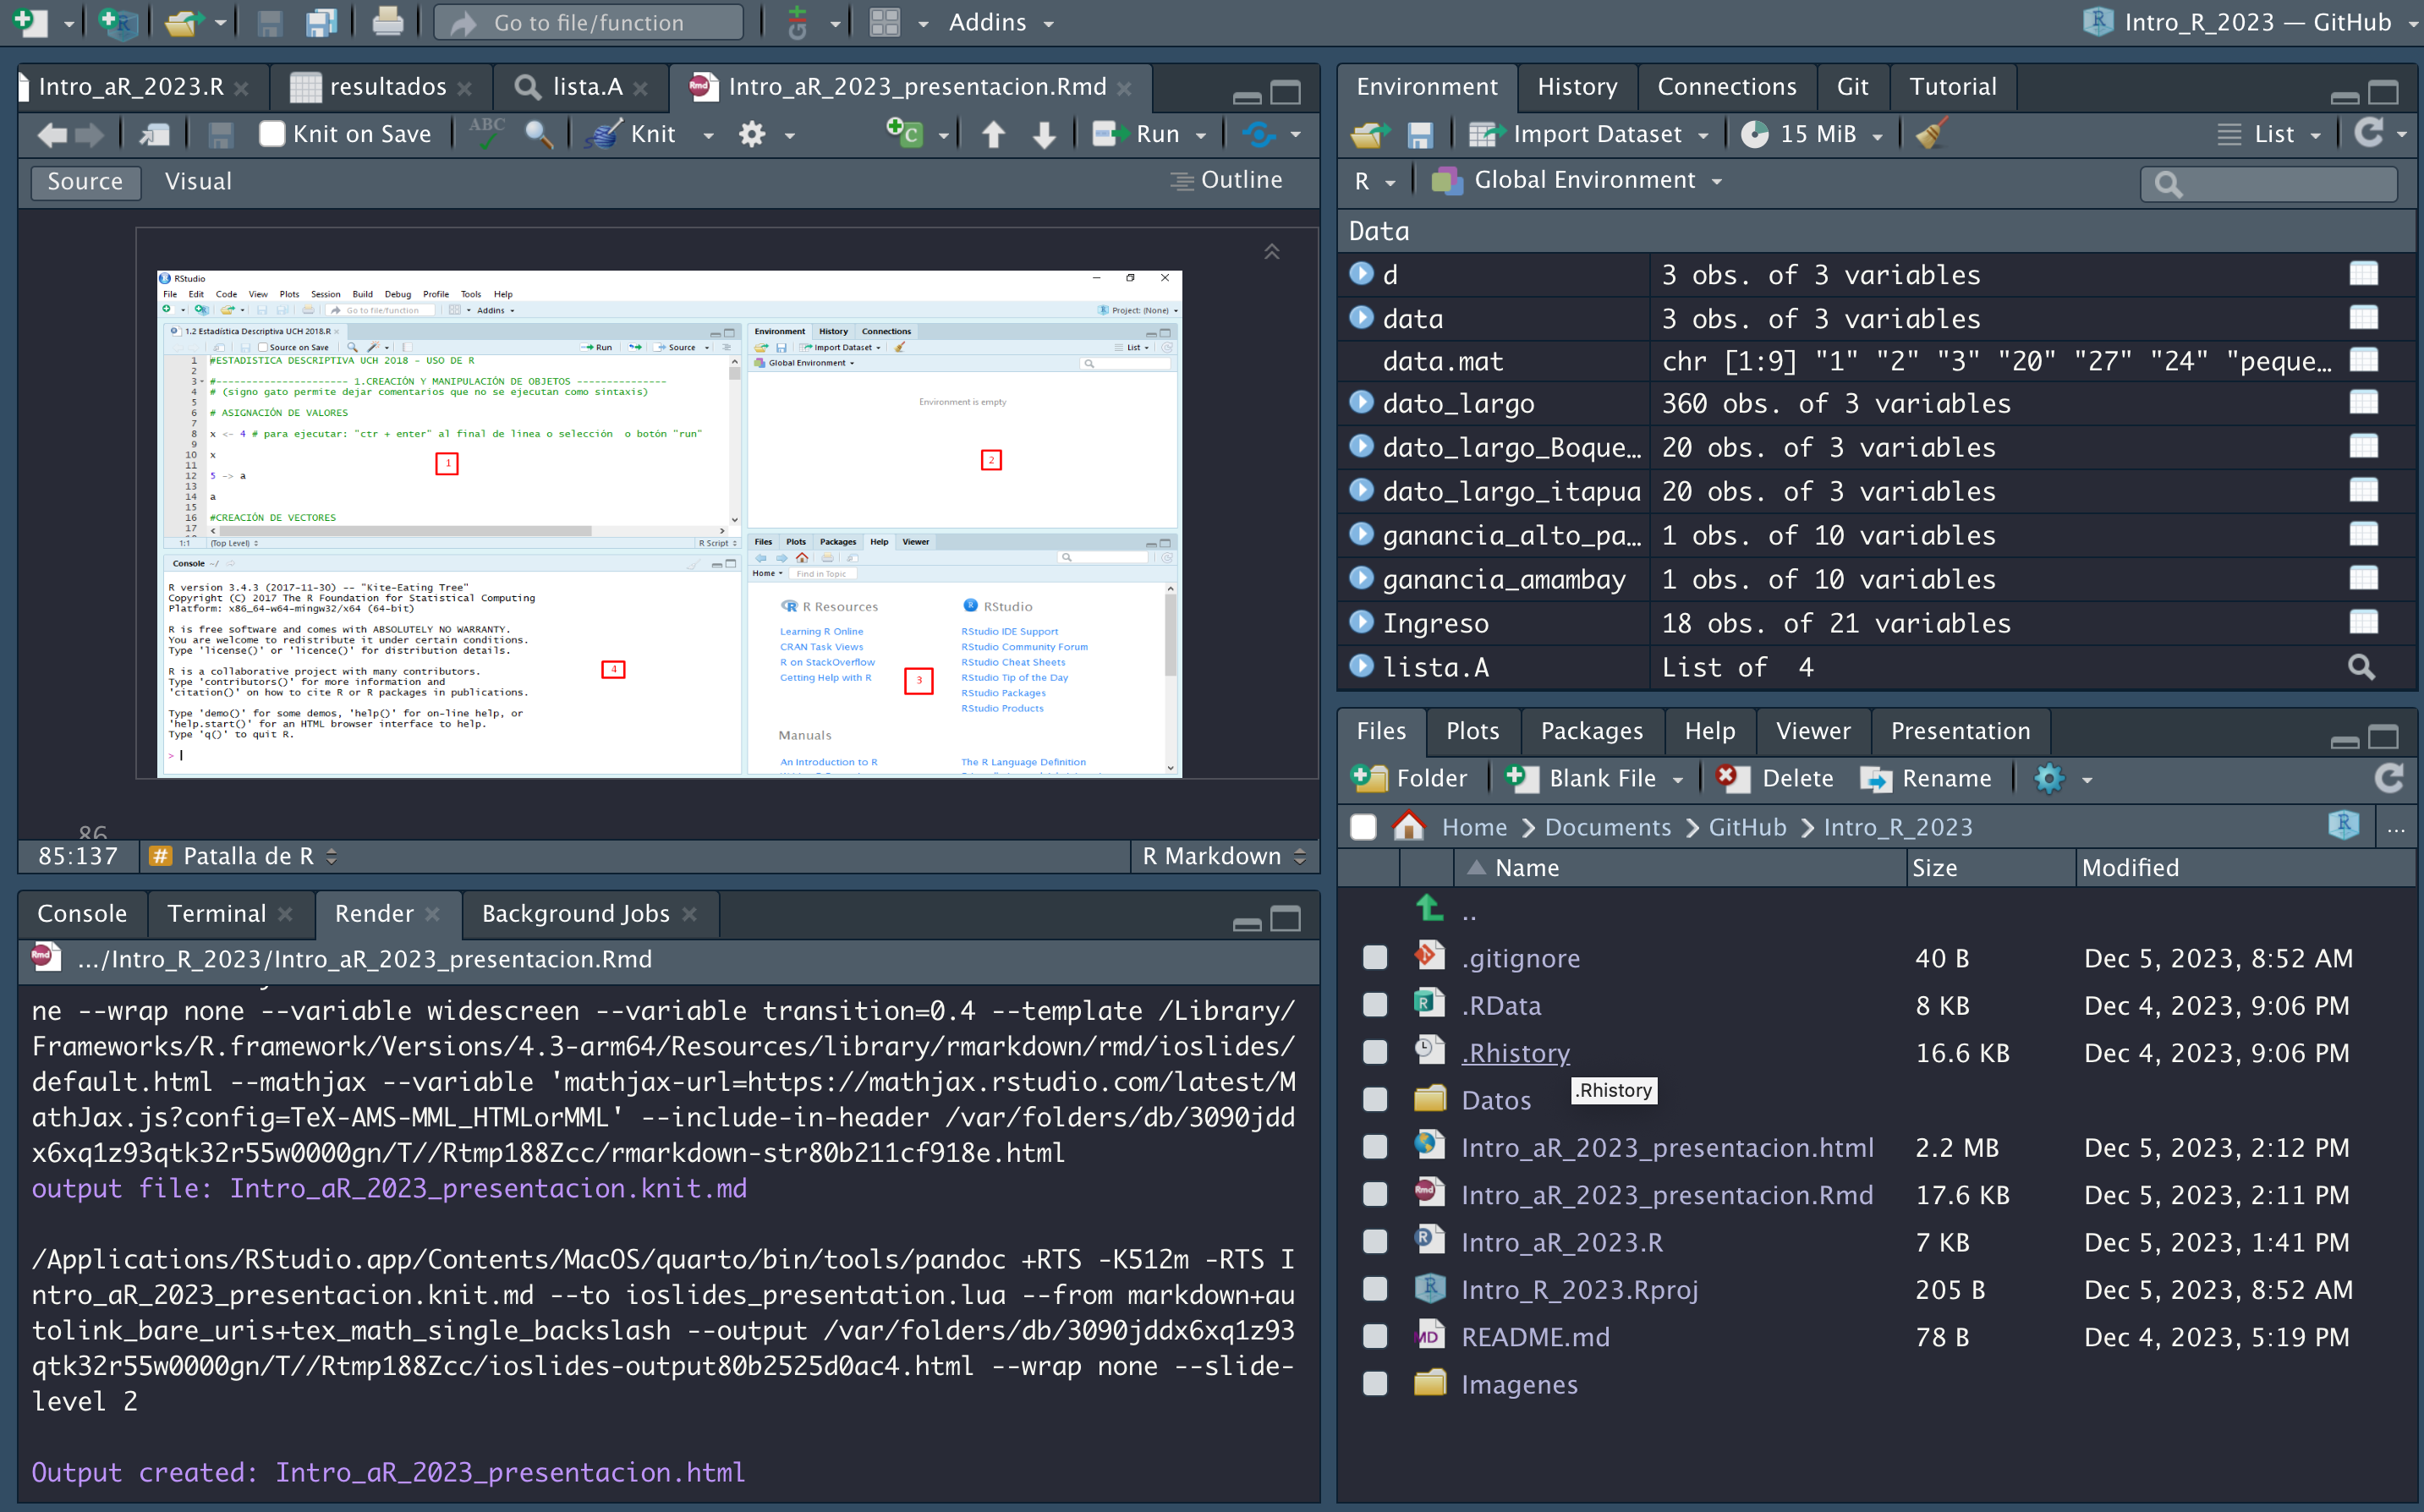
\includegraphics[width=0.8\textwidth,height=0.8\textheight]{Imagenes/RStudio-pantalla.png}
\caption{\url{https://bookdown.org/gboccardo/manual-ED-UCH/uso-basico-de-rstudio.html}}\label{id}
}
\end{figure}
\end{block}

\begin{block}{Directorios de trabajo \textbar{} y comentarios}
\protect\hypertarget{directorios-de-trabajo-y-comentarios}{}
En R, el directorio de trabajo es el lugar en el sistema de archivos
donde R buscará y guardará archivos por defecto.

Comentarios: Proporciona información adicional sobre el propósito o
funcionamiento del código \#

\begin{Shaded}
\begin{Highlighting}[]
\DocumentationTok{\#\#\#\#\#\# Directorios de trabajo}
\CommentTok{\#setwd("\textasciitilde{}/Users/lio/Git/Intro\_R\_2023")  \#Mac}
\FunctionTok{getwd}\NormalTok{() }\CommentTok{\#Donde estamos trabajando?}
\end{Highlighting}
\end{Shaded}

\begin{verbatim}
## [1] "/Users/lio/Git/Intro_R_2023"
\end{verbatim}

\begin{Shaded}
\begin{Highlighting}[]
\CommentTok{\# Comentarios}
\CommentTok{\# comentario}
\end{Highlighting}
\end{Shaded}
\end{block}
\end{frame}

\begin{frame}[fragile]{Paquetes}
\protect\hypertarget{paquetes}{}
Los ``paquetes'' son un conjuntos de herramientas, funciones y datos que
extienden la funcionalidad básica del lenguaje.

\begin{figure}
\hypertarget{id}{%
\centering
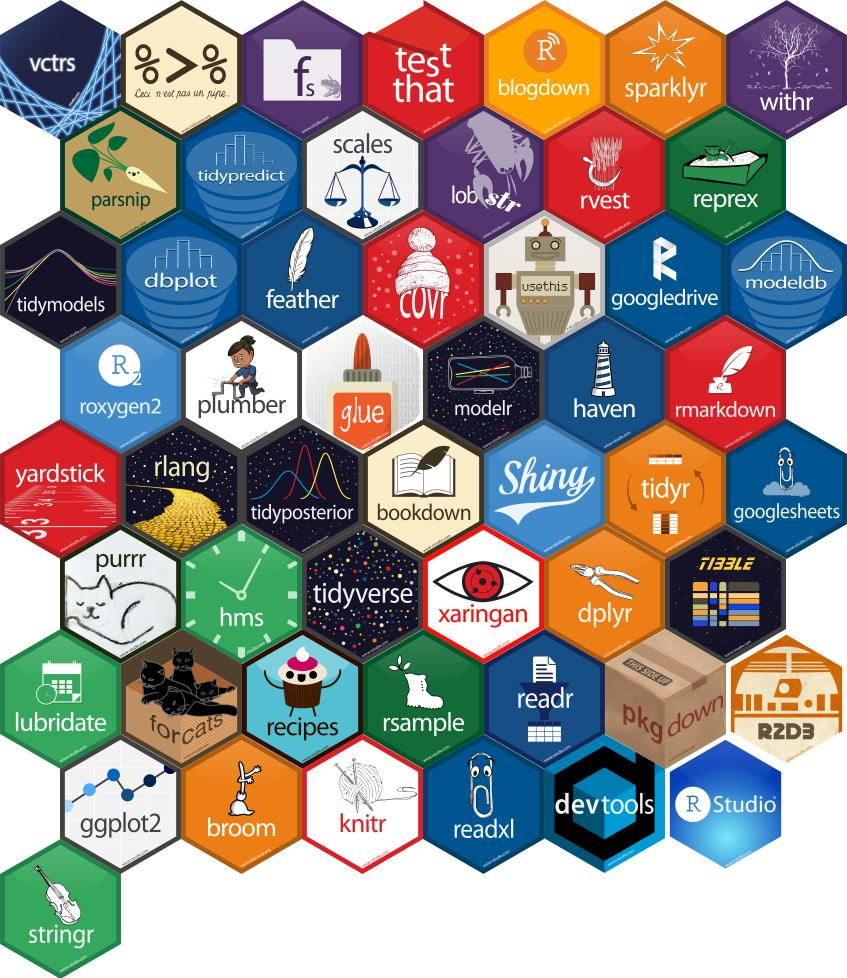
\includegraphics[width=0.4\textwidth,height=0.4\textheight]{Imagenes/Paquetes.jpeg}
\caption{Paquetes}\label{id}
}
\end{figure}

\begin{block}{Paquetes}
\protect\hypertarget{paquetes-1}{}
Los paquetes no se instalan automáticamente con R. Para utilizar un
paquete, primero debes instalarlo.

Una vez instalado, debes cargar un paquete en tu sesión de R para poder
utilizar sus funciones.

\begin{Shaded}
\begin{Highlighting}[]
\CommentTok{\#install.packages("tidyverse")}
\CommentTok{\#install.packages("dplyr")}
\FunctionTok{library}\NormalTok{(tidyverse)}
\FunctionTok{library}\NormalTok{(dplyr) }
\CommentTok{\#update.packages() \#actualiza todos los paquetes que tengas instalados}
\end{Highlighting}
\end{Shaded}
\end{block}
\end{frame}

\begin{frame}{¿Por qué debemos instalar los paquetes?}
\protect\hypertarget{por-quuxe9-debemos-instalar-los-paquetes}{}
\end{frame}

\begin{frame}[fragile]{Ayuda}
\protect\hypertarget{ayuda}{}
En R, el signo de interrogación (?) se utiliza para acceder a la
documentación de una función o de un paquete. Al colocar el signo de
interrogación seguido del nombre de una función o paquete y ejecutar esa
línea de código, R abrirá la documentación correspondiente en la ventana
de ayuda.

\begin{Shaded}
\begin{Highlighting}[]
\NormalTok{?}\FunctionTok{print}\NormalTok{()}
\NormalTok{?lm }\CommentTok{\#Busqueda Simple}
\NormalTok{??lm }\CommentTok{\#Busqueda Amplia }
\end{Highlighting}
\end{Shaded}
\end{frame}

\begin{frame}[fragile]{Operadores}
\protect\hypertarget{operadores}{}
Los operadores son símbolos o palabras clave que realizan operaciones en
variables y valores.

\begin{itemize}
\tightlist
\item
  Operadores de asignación:
\item
  Operadores aritméticos
\item
  Operadores de comparación
\item
  Operadores lógicos
\end{itemize}

\begin{block}{Operadores \textbar{} Operadores de asignación}
\protect\hypertarget{operadores-operadores-de-asignaciuxf3n}{}
\begin{itemize}
\tightlist
\item
  Asignación de variables: \textless- o =
\end{itemize}

\begin{Shaded}
\begin{Highlighting}[]
\NormalTok{variable }\OtherTok{\textless{}{-}} \DecValTok{42}
\NormalTok{variable}
\end{Highlighting}
\end{Shaded}

\begin{verbatim}
## [1] 42
\end{verbatim}
\end{block}

\begin{block}{Operadores \textbar{} Operadores aritméticos}
\protect\hypertarget{operadores-operadores-aritmuxe9ticos}{}
\begin{itemize}
\tightlist
\item
  Suma: +
\item
  Resta: -
\item
  Multiplicación: *
\item
  División: /
\item
  Potenciación: \^{} o **
\item
  Resto de la división entera: \%\%
\item
  Cociente de la división entera: \%/\%
\end{itemize}
\end{block}

\begin{block}{Operadores \textbar{} Operadores aritméticos}
\protect\hypertarget{operadores-operadores-aritmuxe9ticos-1}{}
\begin{Shaded}
\begin{Highlighting}[]
\NormalTok{a }\OtherTok{\textless{}{-}} \DecValTok{10}
\NormalTok{b }\OtherTok{\textless{}{-}} \DecValTok{3}
\NormalTok{suma }\OtherTok{\textless{}{-}}\NormalTok{ a }\SpecialCharTok{+}\NormalTok{ b}
\NormalTok{resta }\OtherTok{\textless{}{-}}\NormalTok{ a }\SpecialCharTok{{-}}\NormalTok{ b}
\NormalTok{multiplicacion }\OtherTok{\textless{}{-}}\NormalTok{ a }\SpecialCharTok{*}\NormalTok{ b}
\NormalTok{division }\OtherTok{\textless{}{-}}\NormalTok{ a }\SpecialCharTok{/}\NormalTok{ b}

\FunctionTok{print}\NormalTok{(suma)}
\end{Highlighting}
\end{Shaded}

\begin{verbatim}
## [1] 13
\end{verbatim}

\begin{Shaded}
\begin{Highlighting}[]
\NormalTok{division}
\end{Highlighting}
\end{Shaded}

\begin{verbatim}
## [1] 3.333333
\end{verbatim}
\end{block}

\begin{block}{Operadores \textbar{} Operadores de comparación}
\protect\hypertarget{operadores-operadores-de-comparaciuxf3n}{}
\begin{itemize}
\tightlist
\item
  Igual a: ==
\item
  No igual a: !=
\item
  Menor que: \textless{}
\item
  Mayor que: \textgreater{}
\item
  Menor o igual que: \textless=
\item
  Mayor o igual que: \textgreater=
\end{itemize}

\begin{Shaded}
\begin{Highlighting}[]
\NormalTok{x }\OtherTok{\textless{}{-}} \DecValTok{5}
\NormalTok{y }\OtherTok{\textless{}{-}} \DecValTok{10}
\NormalTok{resultado }\OtherTok{\textless{}{-}}\NormalTok{ x }\SpecialCharTok{\textgreater{}}\NormalTok{ y}
\FunctionTok{print}\NormalTok{(resultado)}
\end{Highlighting}
\end{Shaded}

\begin{verbatim}
## [1] FALSE
\end{verbatim}
\end{block}

\begin{block}{Operadores \textbar{} Operadores lógicos}
\protect\hypertarget{operadores-operadores-luxf3gicos}{}
\begin{itemize}
\tightlist
\item
  AND lógico: \&
\item
  OR lógico: \textbar{}
\item
  NOT lógico: !
\end{itemize}

\begin{Shaded}
\begin{Highlighting}[]
\NormalTok{condicion1 }\OtherTok{\textless{}{-}} \ConstantTok{TRUE}
\NormalTok{condicion2 }\OtherTok{\textless{}{-}} \ConstantTok{FALSE}
\NormalTok{resultado }\OtherTok{\textless{}{-}}\NormalTok{ condicion1 }\SpecialCharTok{\&}\NormalTok{ condicion2}
\FunctionTok{print}\NormalTok{(resultado)}
\end{Highlighting}
\end{Shaded}

\begin{verbatim}
## [1] FALSE
\end{verbatim}
\end{block}
\end{frame}

\begin{frame}[fragile]{Objetos}
\protect\hypertarget{objetos}{}
En el contexto de R, ``objetos'' se refiere a las estructuras de datos
que almacenan información.

\begin{itemize}
\tightlist
\item
  Funciones
\item
  Vectores
\item
  Matrices
\item
  Listas
\item
  Data Frames (Marco de Datos)
\item
  Factores
\end{itemize}

\begin{block}{Objetos}
\protect\hypertarget{objetos-1}{}
\begin{Shaded}
\begin{Highlighting}[]
\DocumentationTok{\#\# Recuerda que R es un lenguaje sensible a mayúsculas y minúsculas}
\NormalTok{(}\DecValTok{10} \SpecialCharTok{+} \DecValTok{2}\NormalTok{) }\SpecialCharTok{*} \DecValTok{5}
\end{Highlighting}
\end{Shaded}

\begin{verbatim}
## [1] 60
\end{verbatim}

\begin{Shaded}
\begin{Highlighting}[]
\NormalTok{x }\OtherTok{\textless{}{-}}\NormalTok{ (}\DecValTok{10} \SpecialCharTok{+} \DecValTok{2}\NormalTok{) }\SpecialCharTok{*} \DecValTok{5}  \CommentTok{\# \textless{}{-} es equivalente a =}
\NormalTok{x }\OtherTok{\textless{}{-}} \ConstantTok{NA}
\NormalTok{x }\OtherTok{\textless{}{-}} \FunctionTok{c}\NormalTok{(}\DecValTok{8}\NormalTok{,}\DecValTok{9}\NormalTok{,}\DecValTok{10}\NormalTok{,}\DecValTok{12}\NormalTok{,}\DecValTok{14}\NormalTok{,}\DecValTok{10}\NormalTok{,}\DecValTok{13}\NormalTok{,}\DecValTok{10}\NormalTok{,}\DecValTok{9}\NormalTok{)}

\FunctionTok{print}\NormalTok{(x)}
\end{Highlighting}
\end{Shaded}

\begin{verbatim}
## [1]  8  9 10 12 14 10 13 10  9
\end{verbatim}
\end{block}

\begin{block}{Objetos \textbar{} Funciones}
\protect\hypertarget{objetos-funciones}{}
Objetos que contienen código ejecutable.

\begin{longtable}[]{@{}llll@{}}
\toprule\noalign{}
Informacion & Aritmética & Estadistica & Orden \\
\midrule\noalign{}
\endhead
summary(x) & min(x) & sd(x) & rev(x) \\
mode(x) & max(x) & var(x) & unique(x) \\
length(x) & log(x) & median(x) & sort(x) \\
range(x) & sum(x) & mean(x) & rev(sort(x)) \\
\bottomrule\noalign{}
\end{longtable}

\#¿Donde podemos encontrar más funciones?
\end{block}

\begin{block}{Objetos}
\protect\hypertarget{objetos-2}{}
\begin{block}{Vectores: Clase genérica que permite almacenar una
colección de objetos del mismo tipo}
\protect\hypertarget{vectores-clase-genuxe9rica-que-permite-almacenar-una-colecciuxf3n-de-objetos-del-mismo-tipo}{}
\begin{itemize}
\tightlist
\item
  Numericos: Almacenan números reales.
\item
  Enteros: Almacenan números enteros.
\item
  Lógicos: Almacenan valores booleanos (TRUE o FALSE).
\item
  Caracteres: Almacenan texto
\end{itemize}

\begin{Shaded}
\begin{Highlighting}[]
\CommentTok{\# Ejemplos de vectores}
\NormalTok{numeric\_vector }\OtherTok{\textless{}{-}} \FunctionTok{c}\NormalTok{(}\FloatTok{1.5}\NormalTok{, }\FloatTok{2.3}\NormalTok{, }\FloatTok{4.0}\NormalTok{)}
\NormalTok{entero\_vector }\OtherTok{\textless{}{-}} \FunctionTok{c}\NormalTok{(}\DecValTok{1}\NormalTok{, }\DecValTok{2}\NormalTok{, }\DecValTok{3}\NormalTok{)}
\NormalTok{logico\_vector }\OtherTok{\textless{}{-}} \FunctionTok{c}\NormalTok{(}\ConstantTok{TRUE}\NormalTok{, }\ConstantTok{FALSE}\NormalTok{, }\ConstantTok{TRUE}\NormalTok{)}
\NormalTok{caracteres\_vector }\OtherTok{\textless{}{-}} \FunctionTok{c}\NormalTok{(}\StringTok{"uno"}\NormalTok{, }\StringTok{"dos"}\NormalTok{, }\StringTok{"tres"}\NormalTok{)}
\end{Highlighting}
\end{Shaded}
\end{block}
\end{block}

\begin{block}{Objetos \textbar{} Vectores}
\protect\hypertarget{objetos-vectores}{}
\begin{Shaded}
\begin{Highlighting}[]
\NormalTok{peso }\OtherTok{\textless{}{-}} \FunctionTok{c}\NormalTok{(}\DecValTok{60}\NormalTok{, }\DecValTok{72}\NormalTok{, }\DecValTok{57}\NormalTok{, }\DecValTok{90}\NormalTok{, }\DecValTok{95}\NormalTok{, }\DecValTok{72}\NormalTok{) }
\NormalTok{altura }\OtherTok{\textless{}{-}} \FunctionTok{c}\NormalTok{(}\FloatTok{1.75}\NormalTok{, }\FloatTok{1.80}\NormalTok{, }\FloatTok{1.65}\NormalTok{, }\FloatTok{1.90}\NormalTok{, }\FloatTok{1.74}\NormalTok{, }\FloatTok{1.91}\NormalTok{)}
\NormalTok{imc }\OtherTok{\textless{}{-}}\NormalTok{ peso}\SpecialCharTok{/}\NormalTok{altura}\SpecialCharTok{\^{}}\DecValTok{2}

\FunctionTok{print}\NormalTok{(imc)}
\end{Highlighting}
\end{Shaded}

\begin{verbatim}
## [1] 19.59184 22.22222 20.93664 24.93075 31.37799 19.73630
\end{verbatim}
\end{block}

\begin{block}{Objetos}
\protect\hypertarget{objetos-3}{}
Matrices: Arreglos bidimensionales de elementos del mismo tipo.

\begin{Shaded}
\begin{Highlighting}[]
\NormalTok{X }\OtherTok{\textless{}{-}} \FunctionTok{matrix}\NormalTok{(}\FunctionTok{c}\NormalTok{(}\DecValTok{1}\NormalTok{, }\DecValTok{2}\NormalTok{, }\DecValTok{3}\NormalTok{, }\DecValTok{11}\NormalTok{, }\DecValTok{12}\NormalTok{, }\DecValTok{13}\NormalTok{), }\AttributeTok{nrow=}\DecValTok{2}\NormalTok{, }\AttributeTok{ncol=}\DecValTok{3}\NormalTok{, }\AttributeTok{byrow=}\ConstantTok{TRUE}\NormalTok{, }
            \AttributeTok{dimnames=}\FunctionTok{list}\NormalTok{(}\FunctionTok{c}\NormalTok{(}\StringTok{"fila1"}\NormalTok{, }\StringTok{"fila2"}\NormalTok{), }\FunctionTok{c}\NormalTok{(}\StringTok{"C.1"}\NormalTok{, }\StringTok{"C.2"}\NormalTok{, }\StringTok{"C.3"}\NormalTok{)))}

\NormalTok{X}
\end{Highlighting}
\end{Shaded}

\begin{verbatim}
##       C.1 C.2 C.3
## fila1   1   2   3
## fila2  11  12  13
\end{verbatim}

\begin{Shaded}
\begin{Highlighting}[]
\NormalTok{X }\OtherTok{\textless{}{-}} \FunctionTok{matrix}\NormalTok{(}\FunctionTok{c}\NormalTok{(}\DecValTok{10}\NormalTok{, }\DecValTok{10}\NormalTok{, }\DecValTok{10}\NormalTok{, }\DecValTok{10}\NormalTok{, }\DecValTok{10}\NormalTok{, }\DecValTok{10}\NormalTok{), }\AttributeTok{nrow=}\DecValTok{2}\NormalTok{, }\AttributeTok{ncol=}\DecValTok{3}\NormalTok{, }\AttributeTok{byrow=}\ConstantTok{TRUE}\NormalTok{, }
            \AttributeTok{dimnames=}\FunctionTok{list}\NormalTok{(}\FunctionTok{c}\NormalTok{(}\StringTok{"fila1"}\NormalTok{, }\StringTok{"fila2"}\NormalTok{), }\FunctionTok{c}\NormalTok{(}\StringTok{"C.1"}\NormalTok{, }\StringTok{"C.2"}\NormalTok{, }\StringTok{"C.3"}\NormalTok{)))}
\end{Highlighting}
\end{Shaded}
\end{block}

\begin{block}{Objetos \textbar{} Matrices}
\protect\hypertarget{objetos-matrices}{}
\begin{Shaded}
\begin{Highlighting}[]
\FunctionTok{rownames}\NormalTok{(X) }\CommentTok{\#nombre de filas}
\end{Highlighting}
\end{Shaded}

\begin{verbatim}
## [1] "fila1" "fila2"
\end{verbatim}

\begin{Shaded}
\begin{Highlighting}[]
\FunctionTok{colnames}\NormalTok{(X) }\CommentTok{\#nombre de columnas}
\end{Highlighting}
\end{Shaded}

\begin{verbatim}
## [1] "C.1" "C.2" "C.3"
\end{verbatim}

\begin{Shaded}
\begin{Highlighting}[]
\FunctionTok{nrow}\NormalTok{(X) }\CommentTok{\#Numero de filas}
\end{Highlighting}
\end{Shaded}

\begin{verbatim}
## [1] 2
\end{verbatim}

\begin{Shaded}
\begin{Highlighting}[]
\FunctionTok{ncol}\NormalTok{(X) }\CommentTok{\#numero de columnas}
\end{Highlighting}
\end{Shaded}

\begin{verbatim}
## [1] 3
\end{verbatim}

\begin{Shaded}
\begin{Highlighting}[]
\FunctionTok{dim}\NormalTok{(X) }\CommentTok{\#dimensiones}
\end{Highlighting}
\end{Shaded}

\begin{verbatim}
## [1] 2 3
\end{verbatim}

\begin{Shaded}
\begin{Highlighting}[]
\FunctionTok{t}\NormalTok{(X) }\CommentTok{\#trasponer}
\end{Highlighting}
\end{Shaded}

\begin{verbatim}
##     fila1 fila2
## C.1    10    10
## C.2    10    10
## C.3    10    10
\end{verbatim}
\end{block}
\end{frame}

\begin{frame}[fragile]{¿Por qué se muestra la segunda matriz y no la
primera?}
\protect\hypertarget{por-quuxe9-se-muestra-la-segunda-matriz-y-no-la-primera}{}
\begin{block}{Objetos \textbar{} Matrices}
\protect\hypertarget{objetos-matrices-1}{}
Manipulacion de Matrices

\begin{Shaded}
\begin{Highlighting}[]
\NormalTok{C}\FloatTok{.4} \OtherTok{\textless{}{-}} \FunctionTok{c}\NormalTok{(}\DecValTok{100}\NormalTok{, }\DecValTok{1000}\NormalTok{) }\CommentTok{\#crear vector para 4ta columna }
\NormalTok{X1 }\OtherTok{\textless{}{-}} \FunctionTok{cbind}\NormalTok{(X, C}\FloatTok{.4}\NormalTok{) }\CommentTok{\#Agregar 4ta columna a X}
\NormalTok{fila3 }\OtherTok{\textless{}{-}} \FunctionTok{c}\NormalTok{(}\DecValTok{10}\NormalTok{, }\DecValTok{100}\NormalTok{, }\DecValTok{1000}\NormalTok{) }\CommentTok{\#crear fila 3}
\NormalTok{X2 }\OtherTok{\textless{}{-}} \FunctionTok{rbind}\NormalTok{(X, fila3) }\CommentTok{\#agregar fila 3 a X}

\NormalTok{X2}
\end{Highlighting}
\end{Shaded}

\begin{verbatim}
##       C.1 C.2  C.3
## fila1  10  10   10
## fila2  10  10   10
## fila3  10 100 1000
\end{verbatim}
\end{block}

\begin{block}{Objetos \textbar{} Matrices}
\protect\hypertarget{objetos-matrices-2}{}
Manipulacion de Matrices

\begin{Shaded}
\begin{Highlighting}[]
\CommentTok{\#Donde se fue la Columna 4 (C.4)?}
\NormalTok{X2 }\OtherTok{\textless{}{-}} \FunctionTok{rbind}\NormalTok{(X, fila3) }\CommentTok{\#agregar fila 3 a X}
\NormalTok{fila3 }\OtherTok{\textless{}{-}} \FunctionTok{c}\NormalTok{(}\DecValTok{10}\NormalTok{, }\DecValTok{100}\NormalTok{, }\DecValTok{1000}\NormalTok{, }\DecValTok{10000}\NormalTok{) }\CommentTok{\#crear fila 3}
\NormalTok{X3 }\OtherTok{\textless{}{-}} \FunctionTok{rbind}\NormalTok{(X1, fila3) }\CommentTok{\#agregar fila 3 a X}

\NormalTok{X3}
\end{Highlighting}
\end{Shaded}

\begin{verbatim}
##       C.1 C.2  C.3   C.4
## fila1  10  10   10   100
## fila2  10  10   10  1000
## fila3  10 100 1000 10000
\end{verbatim}
\end{block}

\begin{block}{Objetos \textbar{} Lista}
\protect\hypertarget{objetos-lista}{}
Listas: Colecciones ordenadas de objetos de diferentes tipos.

\begin{Shaded}
\begin{Highlighting}[]
\DocumentationTok{\#\# Lista (grupos de cualquier tipo de objeto R)}

\NormalTok{lista\_ejemplo }\OtherTok{\textless{}{-}} \FunctionTok{list}\NormalTok{(numeric\_vector, entero\_vector, logico\_vector, caracteres\_vector)}


\NormalTok{lista\_ejemplo}
\end{Highlighting}
\end{Shaded}

\begin{verbatim}
## [[1]]
## [1] 1.5 2.3 4.0
## 
## [[2]]
## [1] 1 2 3
## 
## [[3]]
## [1]  TRUE FALSE  TRUE
## 
## [[4]]
## [1] "uno"  "dos"  "tres"
\end{verbatim}

\begin{Shaded}
\begin{Highlighting}[]
\NormalTok{lista\_ejemplo[[}\DecValTok{4}\NormalTok{]]}
\end{Highlighting}
\end{Shaded}

\begin{verbatim}
## [1] "uno"  "dos"  "tres"
\end{verbatim}
\end{block}

\begin{block}{Objetos \textbar{} Data Frames}
\protect\hypertarget{objetos-data-frames}{}
Estructuras de datos bidimensionales similares a las matrices, pero
pueden contener columnas de diferentes tipos.

\begin{Shaded}
\begin{Highlighting}[]
\CommentTok{\# Ejemplo de data frame}
\NormalTok{data\_frame\_ejemplo }\OtherTok{\textless{}{-}} \FunctionTok{data.frame}\NormalTok{(}
  \AttributeTok{Nombre =} \FunctionTok{c}\NormalTok{(}\StringTok{"Juan"}\NormalTok{, }\StringTok{"Maria"}\NormalTok{, }\StringTok{"Carlos"}\NormalTok{),}
  \AttributeTok{Edad =} \FunctionTok{c}\NormalTok{(}\DecValTok{25}\NormalTok{, }\DecValTok{30}\NormalTok{, }\DecValTok{22}\NormalTok{),}
  \AttributeTok{Casado =} \FunctionTok{c}\NormalTok{(}\ConstantTok{FALSE}\NormalTok{, }\ConstantTok{TRUE}\NormalTok{, }\ConstantTok{FALSE}\NormalTok{)}
\NormalTok{)}
\NormalTok{data\_frame\_ejemplo}
\end{Highlighting}
\end{Shaded}

\begin{verbatim}
##   Nombre Edad Casado
## 1   Juan   25  FALSE
## 2  Maria   30   TRUE
## 3 Carlos   22  FALSE
\end{verbatim}
\end{block}

\begin{block}{Objetos \textbar{} Data Frames}
\protect\hypertarget{objetos-data-frames-1}{}
Manipulacion de Datos

\begin{Shaded}
\begin{Highlighting}[]
\DocumentationTok{\#\# Marco de datos (Data Frame)}
\NormalTok{data }\OtherTok{\textless{}{-}} \FunctionTok{data.frame}\NormalTok{(}\AttributeTok{alpha=}\DecValTok{1}\SpecialCharTok{:}\DecValTok{3}\NormalTok{, }
                   \AttributeTok{beta=}\DecValTok{4}\SpecialCharTok{:}\DecValTok{6}\NormalTok{, }\AttributeTok{gamma=}\DecValTok{7}\SpecialCharTok{:}\DecValTok{9}\NormalTok{)}
\FunctionTok{names}\NormalTok{(data)[}\DecValTok{3}\NormalTok{] }\OtherTok{\textless{}{-}} \StringTok{"tres"}
\NormalTok{data}\SpecialCharTok{$}\NormalTok{tres }\OtherTok{\textless{}{-}} \ConstantTok{NULL}

\CommentTok{\# Reordenar marco de datos}
\NormalTok{data }\OtherTok{\textless{}{-}} \FunctionTok{data.frame}\NormalTok{(}\AttributeTok{id=}\DecValTok{1}\SpecialCharTok{:}\DecValTok{3}\NormalTok{, }\AttributeTok{peso=}\FunctionTok{c}\NormalTok{(}\DecValTok{50}\NormalTok{, }\DecValTok{90}\NormalTok{, }\DecValTok{75}\NormalTok{), }
\NormalTok{                   tamaño}\OtherTok{=}\FunctionTok{c}\NormalTok{(}\StringTok{"pequeño"}\NormalTok{, }\StringTok{"grande"}\NormalTok{, }\StringTok{"mediano"}\NormalTok{))}
\NormalTok{data[}\FunctionTok{c}\NormalTok{(}\DecValTok{1}\NormalTok{, }\DecValTok{3}\NormalTok{, }\DecValTok{2}\NormalTok{)]}
\end{Highlighting}
\end{Shaded}

\begin{verbatim}
##   id  tamaño peso
## 1  1 pequeño   50
## 2  2  grande   90
## 3  3 mediano   75
\end{verbatim}

\begin{Shaded}
\begin{Highlighting}[]
\NormalTok{data[}\FunctionTok{c}\NormalTok{(}\StringTok{"tamaño"}\NormalTok{, }\StringTok{"id"}\NormalTok{, }\StringTok{"peso"}\NormalTok{)]}
\end{Highlighting}
\end{Shaded}

\begin{verbatim}
##    tamaño id peso
## 1 pequeño  1   50
## 2  grande  2   90
## 3 mediano  3   75
\end{verbatim}
\end{block}

\begin{block}{Objetos \textbar{} Factores}
\protect\hypertarget{objetos-factores}{}
Vectores que representan \textbf{variables categóricas} con
\textbf{niveles} predefinidos.

\begin{Shaded}
\begin{Highlighting}[]
\NormalTok{x }\OtherTok{\textless{}{-}} \FunctionTok{factor}\NormalTok{(}\FunctionTok{c}\NormalTok{(}\StringTok{"alpha"}\NormalTok{, }\StringTok{"beta"}\NormalTok{, }\StringTok{"gamma"}\NormalTok{, }\StringTok{"alpha"}\NormalTok{, }\StringTok{"beta"}\NormalTok{))}
\FunctionTok{levels}\NormalTok{(x) }\CommentTok{\#Distintos Valores unicos que puede tomar un factor}
\end{Highlighting}
\end{Shaded}

\begin{verbatim}
## [1] "alpha" "beta"  "gamma"
\end{verbatim}

\begin{Shaded}
\begin{Highlighting}[]
\FunctionTok{levels}\NormalTok{(x)[}\FunctionTok{levels}\NormalTok{(x)}\SpecialCharTok{==}\StringTok{"beta"}\NormalTok{] }\OtherTok{\textless{}{-}} \StringTok{"dos"} \CommentTok{\#cambiamos beta por dos}
\FunctionTok{levels}\NormalTok{(x)[}\DecValTok{3}\NormalTok{] }\OtherTok{\textless{}{-}} \StringTok{"tres"}  \CommentTok{\#cambiamos el tercer nivel por tres}
\FunctionTok{levels}\NormalTok{(x) }\OtherTok{\textless{}{-}} \FunctionTok{c}\NormalTok{(}\StringTok{"uno"}\NormalTok{, }\StringTok{"dos"}\NormalTok{, }\StringTok{"tres"}\NormalTok{) }\CommentTok{\#cambiamos todos los niveles por el vector}
\end{Highlighting}
\end{Shaded}
\end{block}

\begin{block}{Objetos \textbar{} Manipulaciones}
\protect\hypertarget{objetos-manipulaciones}{}
\begin{Shaded}
\begin{Highlighting}[]
\CommentTok{\# Convertir objetos}
\NormalTok{data }\OtherTok{\textless{}{-}} \FunctionTok{as.matrix}\NormalTok{(data) }\CommentTok{\#Para convertir en Matriz}

\NormalTok{data}
\end{Highlighting}
\end{Shaded}

\begin{verbatim}
##      id  peso tamaño   
## [1,] "1" "50" "pequeño"
## [2,] "2" "90" "grande" 
## [3,] "3" "75" "mediano"
\end{verbatim}

¿Que tipos de datos hay en la matriz?
\end{block}

\begin{block}{Objetos \textbar{} Manipulaciones}
\protect\hypertarget{objetos-manipulaciones-1}{}
\begin{Shaded}
\begin{Highlighting}[]
\CommentTok{\# Convertir objetos}
\NormalTok{data}
\end{Highlighting}
\end{Shaded}

\begin{verbatim}
##      id  peso tamaño   
## [1,] "1" "50" "pequeño"
## [2,] "2" "90" "grande" 
## [3,] "3" "75" "mediano"
\end{verbatim}

\begin{Shaded}
\begin{Highlighting}[]
\NormalTok{data\_1 }\OtherTok{\textless{}{-}} \FunctionTok{as.numeric}\NormalTok{(data) }
\end{Highlighting}
\end{Shaded}

\begin{verbatim}
## Warning: NAs introduced by coercion
\end{verbatim}

\begin{Shaded}
\begin{Highlighting}[]
\CommentTok{\#Para convertir en Matriz}

\NormalTok{data\_1 }
\end{Highlighting}
\end{Shaded}

\begin{verbatim}
## [1]  1  2  3 50 90 75 NA NA NA
\end{verbatim}

\begin{Shaded}
\begin{Highlighting}[]
\CommentTok{\#Que paso con nuestros datos? }
\end{Highlighting}
\end{Shaded}
\end{block}

\begin{block}{Objetos \textbar{} Manipulaciones}
\protect\hypertarget{objetos-manipulaciones-2}{}
\begin{Shaded}
\begin{Highlighting}[]
\CommentTok{\# Convertir objetos}

\FunctionTok{typeof}\NormalTok{(data)}
\end{Highlighting}
\end{Shaded}

\begin{verbatim}
## [1] "character"
\end{verbatim}

\begin{Shaded}
\begin{Highlighting}[]
\NormalTok{data[,}\DecValTok{3}\NormalTok{] }\OtherTok{\textless{}{-}} \FunctionTok{c}\NormalTok{(}\DecValTok{1}\NormalTok{,}\DecValTok{3}\NormalTok{,}\DecValTok{2}\NormalTok{)}

\NormalTok{data}
\end{Highlighting}
\end{Shaded}

\begin{verbatim}
##      id  peso tamaño
## [1,] "1" "50" "1"   
## [2,] "2" "90" "3"   
## [3,] "3" "75" "2"
\end{verbatim}

\begin{Shaded}
\begin{Highlighting}[]
\CommentTok{\# Convertir toda la matriz a tipo numérico}
\NormalTok{data\_numeric }\OtherTok{\textless{}{-}} \FunctionTok{as.numeric}\NormalTok{(data)}

\CommentTok{\# Remodelar la matriz a sus dimensiones originales}
\FunctionTok{dim}\NormalTok{(data\_numeric) }\OtherTok{\textless{}{-}} \FunctionTok{dim}\NormalTok{(data)}

\NormalTok{data\_numeric}
\end{Highlighting}
\end{Shaded}

\begin{verbatim}
##      [,1] [,2] [,3]
## [1,]    1   50    1
## [2,]    2   90    3
## [3,]    3   75    2
\end{verbatim}
\end{block}

\begin{block}{Objetos \textbar{} Manipulaciones}
\protect\hypertarget{objetos-manipulaciones-3}{}
\begin{Shaded}
\begin{Highlighting}[]
\NormalTok{x }\OtherTok{\textless{}{-}} \DecValTok{1}\SpecialCharTok{:}\DecValTok{20} \CommentTok{\#Creamos un Objeto}
\NormalTok{x[}\DecValTok{3}\NormalTok{] }\OtherTok{\textless{}{-}} \DecValTok{100} \CommentTok{\#introducir 100 en el lugar 3}

\NormalTok{x}
\end{Highlighting}
\end{Shaded}

\begin{verbatim}
##  [1]   1   2 100   4   5   6   7   8   9  10  11  12  13  14  15  16  17  18  19
## [20]  20
\end{verbatim}

\begin{Shaded}
\begin{Highlighting}[]
\NormalTok{x[}\FunctionTok{c}\NormalTok{(}\DecValTok{2}\NormalTok{, }\DecValTok{4}\NormalTok{)] }\OtherTok{\textless{}{-}} \DecValTok{111} \CommentTok{\#Introcir 111 en el lugar 2 y 4}

\NormalTok{x}
\end{Highlighting}
\end{Shaded}

\begin{verbatim}
##  [1]   1 111 100 111   5   6   7   8   9  10  11  12  13  14  15  16  17  18  19
## [20]  20
\end{verbatim}

\begin{Shaded}
\begin{Highlighting}[]
\CommentTok{\#Que tipo de objeto es x?}
\end{Highlighting}
\end{Shaded}
\end{block}
\end{frame}

\begin{frame}[fragile]{Indexacion}
\protect\hypertarget{indexacion}{}
La indexación en R se refiere a la forma en que accedemos a elementos
específicos en un objeto de datos, como vectores, matrices, listas o
data frames.

\url{https://rpubs.com/adiedrichs/basicIndexInR}

\begin{Shaded}
\begin{Highlighting}[]
\NormalTok{iris}
\end{Highlighting}
\end{Shaded}

\begin{verbatim}
##     Sepal.Length Sepal.Width Petal.Length Petal.Width    Species
## 1            5.1         3.5          1.4         0.2     setosa
## 2            4.9         3.0          1.4         0.2     setosa
## 3            4.7         3.2          1.3         0.2     setosa
## 4            4.6         3.1          1.5         0.2     setosa
## 5            5.0         3.6          1.4         0.2     setosa
## 6            5.4         3.9          1.7         0.4     setosa
## 7            4.6         3.4          1.4         0.3     setosa
## 8            5.0         3.4          1.5         0.2     setosa
## 9            4.4         2.9          1.4         0.2     setosa
## 10           4.9         3.1          1.5         0.1     setosa
## 11           5.4         3.7          1.5         0.2     setosa
## 12           4.8         3.4          1.6         0.2     setosa
## 13           4.8         3.0          1.4         0.1     setosa
## 14           4.3         3.0          1.1         0.1     setosa
## 15           5.8         4.0          1.2         0.2     setosa
## 16           5.7         4.4          1.5         0.4     setosa
## 17           5.4         3.9          1.3         0.4     setosa
## 18           5.1         3.5          1.4         0.3     setosa
## 19           5.7         3.8          1.7         0.3     setosa
## 20           5.1         3.8          1.5         0.3     setosa
## 21           5.4         3.4          1.7         0.2     setosa
## 22           5.1         3.7          1.5         0.4     setosa
## 23           4.6         3.6          1.0         0.2     setosa
## 24           5.1         3.3          1.7         0.5     setosa
## 25           4.8         3.4          1.9         0.2     setosa
## 26           5.0         3.0          1.6         0.2     setosa
## 27           5.0         3.4          1.6         0.4     setosa
## 28           5.2         3.5          1.5         0.2     setosa
## 29           5.2         3.4          1.4         0.2     setosa
## 30           4.7         3.2          1.6         0.2     setosa
## 31           4.8         3.1          1.6         0.2     setosa
## 32           5.4         3.4          1.5         0.4     setosa
## 33           5.2         4.1          1.5         0.1     setosa
## 34           5.5         4.2          1.4         0.2     setosa
## 35           4.9         3.1          1.5         0.2     setosa
## 36           5.0         3.2          1.2         0.2     setosa
## 37           5.5         3.5          1.3         0.2     setosa
## 38           4.9         3.6          1.4         0.1     setosa
## 39           4.4         3.0          1.3         0.2     setosa
## 40           5.1         3.4          1.5         0.2     setosa
## 41           5.0         3.5          1.3         0.3     setosa
## 42           4.5         2.3          1.3         0.3     setosa
## 43           4.4         3.2          1.3         0.2     setosa
## 44           5.0         3.5          1.6         0.6     setosa
## 45           5.1         3.8          1.9         0.4     setosa
## 46           4.8         3.0          1.4         0.3     setosa
## 47           5.1         3.8          1.6         0.2     setosa
## 48           4.6         3.2          1.4         0.2     setosa
## 49           5.3         3.7          1.5         0.2     setosa
## 50           5.0         3.3          1.4         0.2     setosa
## 51           7.0         3.2          4.7         1.4 versicolor
## 52           6.4         3.2          4.5         1.5 versicolor
## 53           6.9         3.1          4.9         1.5 versicolor
## 54           5.5         2.3          4.0         1.3 versicolor
## 55           6.5         2.8          4.6         1.5 versicolor
## 56           5.7         2.8          4.5         1.3 versicolor
## 57           6.3         3.3          4.7         1.6 versicolor
## 58           4.9         2.4          3.3         1.0 versicolor
## 59           6.6         2.9          4.6         1.3 versicolor
## 60           5.2         2.7          3.9         1.4 versicolor
## 61           5.0         2.0          3.5         1.0 versicolor
## 62           5.9         3.0          4.2         1.5 versicolor
## 63           6.0         2.2          4.0         1.0 versicolor
## 64           6.1         2.9          4.7         1.4 versicolor
## 65           5.6         2.9          3.6         1.3 versicolor
## 66           6.7         3.1          4.4         1.4 versicolor
## 67           5.6         3.0          4.5         1.5 versicolor
## 68           5.8         2.7          4.1         1.0 versicolor
## 69           6.2         2.2          4.5         1.5 versicolor
## 70           5.6         2.5          3.9         1.1 versicolor
## 71           5.9         3.2          4.8         1.8 versicolor
## 72           6.1         2.8          4.0         1.3 versicolor
## 73           6.3         2.5          4.9         1.5 versicolor
## 74           6.1         2.8          4.7         1.2 versicolor
## 75           6.4         2.9          4.3         1.3 versicolor
## 76           6.6         3.0          4.4         1.4 versicolor
## 77           6.8         2.8          4.8         1.4 versicolor
## 78           6.7         3.0          5.0         1.7 versicolor
## 79           6.0         2.9          4.5         1.5 versicolor
## 80           5.7         2.6          3.5         1.0 versicolor
## 81           5.5         2.4          3.8         1.1 versicolor
## 82           5.5         2.4          3.7         1.0 versicolor
## 83           5.8         2.7          3.9         1.2 versicolor
## 84           6.0         2.7          5.1         1.6 versicolor
## 85           5.4         3.0          4.5         1.5 versicolor
## 86           6.0         3.4          4.5         1.6 versicolor
## 87           6.7         3.1          4.7         1.5 versicolor
## 88           6.3         2.3          4.4         1.3 versicolor
## 89           5.6         3.0          4.1         1.3 versicolor
## 90           5.5         2.5          4.0         1.3 versicolor
## 91           5.5         2.6          4.4         1.2 versicolor
## 92           6.1         3.0          4.6         1.4 versicolor
## 93           5.8         2.6          4.0         1.2 versicolor
## 94           5.0         2.3          3.3         1.0 versicolor
## 95           5.6         2.7          4.2         1.3 versicolor
## 96           5.7         3.0          4.2         1.2 versicolor
## 97           5.7         2.9          4.2         1.3 versicolor
## 98           6.2         2.9          4.3         1.3 versicolor
## 99           5.1         2.5          3.0         1.1 versicolor
## 100          5.7         2.8          4.1         1.3 versicolor
## 101          6.3         3.3          6.0         2.5  virginica
## 102          5.8         2.7          5.1         1.9  virginica
## 103          7.1         3.0          5.9         2.1  virginica
## 104          6.3         2.9          5.6         1.8  virginica
## 105          6.5         3.0          5.8         2.2  virginica
## 106          7.6         3.0          6.6         2.1  virginica
## 107          4.9         2.5          4.5         1.7  virginica
## 108          7.3         2.9          6.3         1.8  virginica
## 109          6.7         2.5          5.8         1.8  virginica
## 110          7.2         3.6          6.1         2.5  virginica
## 111          6.5         3.2          5.1         2.0  virginica
## 112          6.4         2.7          5.3         1.9  virginica
## 113          6.8         3.0          5.5         2.1  virginica
## 114          5.7         2.5          5.0         2.0  virginica
## 115          5.8         2.8          5.1         2.4  virginica
## 116          6.4         3.2          5.3         2.3  virginica
## 117          6.5         3.0          5.5         1.8  virginica
## 118          7.7         3.8          6.7         2.2  virginica
## 119          7.7         2.6          6.9         2.3  virginica
## 120          6.0         2.2          5.0         1.5  virginica
## 121          6.9         3.2          5.7         2.3  virginica
## 122          5.6         2.8          4.9         2.0  virginica
## 123          7.7         2.8          6.7         2.0  virginica
## 124          6.3         2.7          4.9         1.8  virginica
## 125          6.7         3.3          5.7         2.1  virginica
## 126          7.2         3.2          6.0         1.8  virginica
## 127          6.2         2.8          4.8         1.8  virginica
## 128          6.1         3.0          4.9         1.8  virginica
## 129          6.4         2.8          5.6         2.1  virginica
## 130          7.2         3.0          5.8         1.6  virginica
## 131          7.4         2.8          6.1         1.9  virginica
## 132          7.9         3.8          6.4         2.0  virginica
## 133          6.4         2.8          5.6         2.2  virginica
## 134          6.3         2.8          5.1         1.5  virginica
## 135          6.1         2.6          5.6         1.4  virginica
## 136          7.7         3.0          6.1         2.3  virginica
## 137          6.3         3.4          5.6         2.4  virginica
## 138          6.4         3.1          5.5         1.8  virginica
## 139          6.0         3.0          4.8         1.8  virginica
## 140          6.9         3.1          5.4         2.1  virginica
## 141          6.7         3.1          5.6         2.4  virginica
## 142          6.9         3.1          5.1         2.3  virginica
## 143          5.8         2.7          5.1         1.9  virginica
## 144          6.8         3.2          5.9         2.3  virginica
## 145          6.7         3.3          5.7         2.5  virginica
## 146          6.7         3.0          5.2         2.3  virginica
## 147          6.3         2.5          5.0         1.9  virginica
## 148          6.5         3.0          5.2         2.0  virginica
## 149          6.2         3.4          5.4         2.3  virginica
## 150          5.9         3.0          5.1         1.8  virginica
\end{verbatim}

\begin{block}{Indexacion}
\protect\hypertarget{indexacion-1}{}
\begin{figure}
\hypertarget{id}{%
\centering
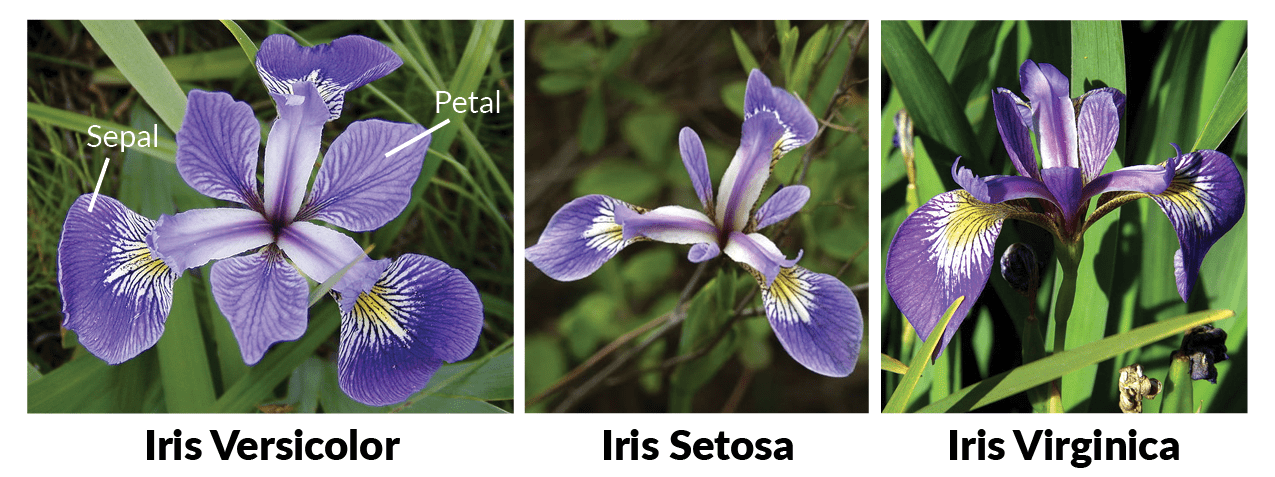
\includegraphics[width=0.9\textwidth,height=0.9\textheight]{Imagenes/iris.png}
\caption{\url{http://www.lac.inpe.br/~rafael.santos/Docs/CAP394/WholeStory-Iris.html}}\label{id}
}
\end{figure}
\end{block}

\begin{block}{Indexacion}
\protect\hypertarget{indexacion-2}{}
\begin{Shaded}
\begin{Highlighting}[]
\FunctionTok{head}\NormalTok{(iris[}\DecValTok{3}\NormalTok{]) }\CommentTok{\#columna 3}
\end{Highlighting}
\end{Shaded}

\begin{verbatim}
##   Petal.Length
## 1          1.4
## 2          1.4
## 3          1.3
## 4          1.5
## 5          1.4
## 6          1.7
\end{verbatim}

\begin{Shaded}
\begin{Highlighting}[]
\FunctionTok{head}\NormalTok{(iris[}\FunctionTok{c}\NormalTok{(}\DecValTok{1}\NormalTok{, }\DecValTok{2}\NormalTok{)])}
\end{Highlighting}
\end{Shaded}

\begin{verbatim}
##   Sepal.Length Sepal.Width
## 1          5.1         3.5
## 2          4.9         3.0
## 3          4.7         3.2
## 4          4.6         3.1
## 5          5.0         3.6
## 6          5.4         3.9
\end{verbatim}

\begin{Shaded}
\begin{Highlighting}[]
\FunctionTok{head}\NormalTok{(iris[}\DecValTok{1}\NormalTok{,]) }\CommentTok{\#Numero de fila}
\end{Highlighting}
\end{Shaded}

\begin{verbatim}
##   Sepal.Length Sepal.Width Petal.Length Petal.Width Species
## 1          5.1         3.5          1.4         0.2  setosa
\end{verbatim}

\begin{Shaded}
\begin{Highlighting}[]
\FunctionTok{head}\NormalTok{(iris[,}\DecValTok{4}\NormalTok{])}\CommentTok{\#Datos en Columna 4}
\end{Highlighting}
\end{Shaded}

\begin{verbatim}
## [1] 0.2 0.2 0.2 0.2 0.2 0.4
\end{verbatim}

\begin{Shaded}
\begin{Highlighting}[]
\FunctionTok{head}\NormalTok{(iris[}\DecValTok{15}\NormalTok{,}\DecValTok{3}\NormalTok{])  }\CommentTok{\#Numero de fila y columna}
\end{Highlighting}
\end{Shaded}

\begin{verbatim}
## [1] 1.2
\end{verbatim}
\end{block}

\begin{block}{Indexacion}
\protect\hypertarget{indexacion-3}{}
Creamos dos vectores

\begin{Shaded}
\begin{Highlighting}[]
\NormalTok{Sepalos\_largo }\OtherTok{\textless{}{-}}\NormalTok{ iris}\SpecialCharTok{$}\NormalTok{Sepal.Length }\CommentTok{\#en cm}
\NormalTok{Petalos\_largo }\OtherTok{\textless{}{-}}\NormalTok{ iris}\SpecialCharTok{$}\NormalTok{Petal.Length }\CommentTok{\#en cm}

\CommentTok{\#Selleccionar vectores}
\NormalTok{Sepalos\_largo }\SpecialCharTok{\textgreater{}} \DecValTok{6}
\end{Highlighting}
\end{Shaded}

\begin{verbatim}
##   [1] FALSE FALSE FALSE FALSE FALSE FALSE FALSE FALSE FALSE FALSE FALSE FALSE
##  [13] FALSE FALSE FALSE FALSE FALSE FALSE FALSE FALSE FALSE FALSE FALSE FALSE
##  [25] FALSE FALSE FALSE FALSE FALSE FALSE FALSE FALSE FALSE FALSE FALSE FALSE
##  [37] FALSE FALSE FALSE FALSE FALSE FALSE FALSE FALSE FALSE FALSE FALSE FALSE
##  [49] FALSE FALSE  TRUE  TRUE  TRUE FALSE  TRUE FALSE  TRUE FALSE  TRUE FALSE
##  [61] FALSE FALSE FALSE  TRUE FALSE  TRUE FALSE FALSE  TRUE FALSE FALSE  TRUE
##  [73]  TRUE  TRUE  TRUE  TRUE  TRUE  TRUE FALSE FALSE FALSE FALSE FALSE FALSE
##  [85] FALSE FALSE  TRUE  TRUE FALSE FALSE FALSE  TRUE FALSE FALSE FALSE FALSE
##  [97] FALSE  TRUE FALSE FALSE  TRUE FALSE  TRUE  TRUE  TRUE  TRUE FALSE  TRUE
## [109]  TRUE  TRUE  TRUE  TRUE  TRUE FALSE FALSE  TRUE  TRUE  TRUE  TRUE FALSE
## [121]  TRUE FALSE  TRUE  TRUE  TRUE  TRUE  TRUE  TRUE  TRUE  TRUE  TRUE  TRUE
## [133]  TRUE  TRUE  TRUE  TRUE  TRUE  TRUE FALSE  TRUE  TRUE  TRUE FALSE  TRUE
## [145]  TRUE  TRUE  TRUE  TRUE  TRUE FALSE
\end{verbatim}

\begin{Shaded}
\begin{Highlighting}[]
\NormalTok{Sepalos\_largo[Sepalos\_largo }\SpecialCharTok{\textgreater{}} \DecValTok{6}\NormalTok{]}
\end{Highlighting}
\end{Shaded}

\begin{verbatim}
##  [1] 7.0 6.4 6.9 6.5 6.3 6.6 6.1 6.7 6.2 6.1 6.3 6.1 6.4 6.6 6.8 6.7 6.7 6.3 6.1
## [20] 6.2 6.3 7.1 6.3 6.5 7.6 7.3 6.7 7.2 6.5 6.4 6.8 6.4 6.5 7.7 7.7 6.9 7.7 6.3
## [39] 6.7 7.2 6.2 6.1 6.4 7.2 7.4 7.9 6.4 6.3 6.1 7.7 6.3 6.4 6.9 6.7 6.9 6.8 6.7
## [58] 6.7 6.3 6.5 6.2
\end{verbatim}
\end{block}

\begin{block}{Indexacion}
\protect\hypertarget{indexacion-4}{}
\begin{Shaded}
\begin{Highlighting}[]
\NormalTok{Petalos\_largo[Petalos\_largo }\SpecialCharTok{\textgreater{}} \DecValTok{5}\NormalTok{]}
\end{Highlighting}
\end{Shaded}

\begin{verbatim}
##  [1] 5.1 6.0 5.1 5.9 5.6 5.8 6.6 6.3 5.8 6.1 5.1 5.3 5.5 5.1 5.3 5.5 6.7 6.9 5.7
## [20] 6.7 5.7 6.0 5.6 5.8 6.1 6.4 5.6 5.1 5.6 6.1 5.6 5.5 5.4 5.6 5.1 5.1 5.9 5.7
## [39] 5.2 5.2 5.4 5.1
\end{verbatim}

\begin{Shaded}
\begin{Highlighting}[]
\NormalTok{Petalos\_largo[Sepalos\_largo }\SpecialCharTok{\textgreater{}} \DecValTok{6} \SpecialCharTok{\&}\NormalTok{ Petalos\_largo }\SpecialCharTok{\textgreater{}} \DecValTok{6}\NormalTok{]}
\end{Highlighting}
\end{Shaded}

\begin{verbatim}
## [1] 6.6 6.3 6.1 6.7 6.9 6.7 6.1 6.4 6.1
\end{verbatim}

\begin{Shaded}
\begin{Highlighting}[]
\NormalTok{Petalos\_largo[Sepalos\_largo }\SpecialCharTok{\textgreater{}} \DecValTok{6} \SpecialCharTok{\&}\NormalTok{ Petalos\_largo }\SpecialCharTok{\textgreater{}} \DecValTok{6}\NormalTok{]}
\end{Highlighting}
\end{Shaded}

\begin{verbatim}
## [1] 6.6 6.3 6.1 6.7 6.9 6.7 6.1 6.4 6.1
\end{verbatim}
\end{block}

\begin{block}{Generacion de Datos}
\protect\hypertarget{generacion-de-datos}{}
\begin{Shaded}
\begin{Highlighting}[]
\DecValTok{1}\SpecialCharTok{:}\DecValTok{10}
\end{Highlighting}
\end{Shaded}

\begin{verbatim}
##  [1]  1  2  3  4  5  6  7  8  9 10
\end{verbatim}

\begin{Shaded}
\begin{Highlighting}[]
\FunctionTok{seq}\NormalTok{(}\AttributeTok{from=}\DecValTok{1}\NormalTok{, }\AttributeTok{to=}\DecValTok{10}\NormalTok{, }\AttributeTok{by=}\DecValTok{1}\NormalTok{)}
\end{Highlighting}
\end{Shaded}

\begin{verbatim}
##  [1]  1  2  3  4  5  6  7  8  9 10
\end{verbatim}

\begin{Shaded}
\begin{Highlighting}[]
\FunctionTok{seq}\NormalTok{(}\DecValTok{1}\NormalTok{, }\DecValTok{10}\NormalTok{, }\DecValTok{1}\NormalTok{)}
\end{Highlighting}
\end{Shaded}

\begin{verbatim}
##  [1]  1  2  3  4  5  6  7  8  9 10
\end{verbatim}

\begin{Shaded}
\begin{Highlighting}[]
\FunctionTok{seq}\NormalTok{(}\AttributeTok{length=}\DecValTok{9}\NormalTok{, }\AttributeTok{from=}\DecValTok{1}\NormalTok{, }\AttributeTok{to=}\DecValTok{5}\NormalTok{)}
\end{Highlighting}
\end{Shaded}

\begin{verbatim}
## [1] 1.0 1.5 2.0 2.5 3.0 3.5 4.0 4.5 5.0
\end{verbatim}

\begin{Shaded}
\begin{Highlighting}[]
\FunctionTok{seq}\NormalTok{(}\DecValTok{1}\NormalTok{, }\DecValTok{3}\NormalTok{, }\AttributeTok{length=}\DecValTok{7}\NormalTok{)}
\end{Highlighting}
\end{Shaded}

\begin{verbatim}
## [1] 1.000000 1.333333 1.666667 2.000000 2.333333 2.666667 3.000000
\end{verbatim}

\begin{Shaded}
\begin{Highlighting}[]
\FunctionTok{c}\NormalTok{(}\DecValTok{1}\NormalTok{, }\DecValTok{2}\NormalTok{, }\DecValTok{3}\NormalTok{, }\DecValTok{4}\NormalTok{, }\DecValTok{5}\NormalTok{)}
\end{Highlighting}
\end{Shaded}

\begin{verbatim}
## [1] 1 2 3 4 5
\end{verbatim}

\begin{Shaded}
\begin{Highlighting}[]
\FunctionTok{rep}\NormalTok{(}\DecValTok{1}\NormalTok{, }\DecValTok{30}\NormalTok{)}
\end{Highlighting}
\end{Shaded}

\begin{verbatim}
##  [1] 1 1 1 1 1 1 1 1 1 1 1 1 1 1 1 1 1 1 1 1 1 1 1 1 1 1 1 1 1 1
\end{verbatim}

\begin{Shaded}
\begin{Highlighting}[]
\FunctionTok{rep}\NormalTok{(}\DecValTok{1}\SpecialCharTok{:}\DecValTok{3}\NormalTok{, }\DecValTok{10}\NormalTok{)}
\end{Highlighting}
\end{Shaded}

\begin{verbatim}
##  [1] 1 2 3 1 2 3 1 2 3 1 2 3 1 2 3 1 2 3 1 2 3 1 2 3 1 2 3 1 2 3
\end{verbatim}
\end{block}

\begin{block}{Generacion de Datos}
\protect\hypertarget{generacion-de-datos-1}{}
Relevamiento de rindes, (50 parcelas, media de 2,8 t/ha, sd=0,8)

\begin{Shaded}
\begin{Highlighting}[]
\FunctionTok{rnorm}\NormalTok{(}\DecValTok{50}\NormalTok{,}\FloatTok{2.8}\NormalTok{,}\FloatTok{0.8}\NormalTok{) }\CommentTok{\#n = observaciones, mean = media, sd = desviacion standart}
\end{Highlighting}
\end{Shaded}

\begin{verbatim}
##  [1] 2.9313541 1.8358737 0.9548969 3.3687367 2.2539779 3.2182638 3.1268990
##  [8] 3.5309060 2.0713870 2.5748312 0.3473315 3.2275921 3.5129653 3.2783886
## [15] 2.9154066 2.5726426 2.7284152 4.7241191 3.3386915 3.2136631 2.4757564
## [22] 2.5845417 3.3475550 2.6790140 4.4180050 1.3374493 3.4575844 0.3351301
## [29] 2.4671285 1.7115935 2.4600301 1.7658684 2.7729162 2.9899768 1.8314520
## [36] 2.6395882 1.3386603 2.4474035 1.3646786 2.5162759 1.0939675 2.6303971
## [43] 2.2306006 1.8945392 2.6612903 1.7150900 3.1500022 1.9872801 2.9884093
## [50] 4.3186408
\end{verbatim}

\begin{Shaded}
\begin{Highlighting}[]
\CommentTok{\#https://www.tutorialspoint.com/r/r\_normal\_distribution.htm}
\end{Highlighting}
\end{Shaded}
\end{block}

\begin{block}{Generacion de Datos}
\protect\hypertarget{generacion-de-datos-2}{}
\includegraphics{Intro_aR_2023_presentacion_files/figure-beamer/unnamed-chunk-29-1.pdf}
\end{block}

\begin{block}{Graficos}
\protect\hypertarget{graficos}{}
\begin{Shaded}
\begin{Highlighting}[]
\FunctionTok{plot}\NormalTok{(Sepalos\_largo)}
\end{Highlighting}
\end{Shaded}

\includegraphics{Intro_aR_2023_presentacion_files/figure-beamer/unnamed-chunk-30-1.pdf}
\end{block}

\begin{block}{Graficos}
\protect\hypertarget{graficos-1}{}
\begin{Shaded}
\begin{Highlighting}[]
\FunctionTok{plot}\NormalTok{(Sepalos\_largo, }\AttributeTok{type=}\StringTok{"p"}\NormalTok{)}
\end{Highlighting}
\end{Shaded}

\includegraphics{Intro_aR_2023_presentacion_files/figure-beamer/unnamed-chunk-31-1.pdf}
\end{block}

\begin{block}{Graficos}
\protect\hypertarget{graficos-2}{}
Relacion Lineal

\begin{Shaded}
\begin{Highlighting}[]
\FunctionTok{plot}\NormalTok{(Sepalos\_largo}\SpecialCharTok{\textasciitilde{}}\NormalTok{Petalos\_largo, }\AttributeTok{main=}\StringTok{"Iris"}\NormalTok{, }\AttributeTok{xlab=}\StringTok{"Sepalos (cm)"}\NormalTok{, }\AttributeTok{ylab=}\StringTok{"Petalos (cm)"}\NormalTok{)}
\end{Highlighting}
\end{Shaded}

\includegraphics{Intro_aR_2023_presentacion_files/figure-beamer/unnamed-chunk-32-1.pdf}
\end{block}

\begin{block}{Graficos}
\protect\hypertarget{graficos-3}{}
histograma

\begin{Shaded}
\begin{Highlighting}[]
\FunctionTok{hist}\NormalTok{(}\FunctionTok{rnorm}\NormalTok{(}\DecValTok{50}\NormalTok{,}\FloatTok{2.8}\NormalTok{,}\FloatTok{0.8}\NormalTok{))}
\end{Highlighting}
\end{Shaded}

\includegraphics{Intro_aR_2023_presentacion_files/figure-beamer/unnamed-chunk-33-1.pdf}
\end{block}
\end{frame}

\begin{frame}[fragile]{tidyverse}
\protect\hypertarget{tidyverse}{}
\texttt{tidyverse} es un conjunto de paquetes de R diseñados para
trabajar de manera integrada y coherente en el análisis de datos.

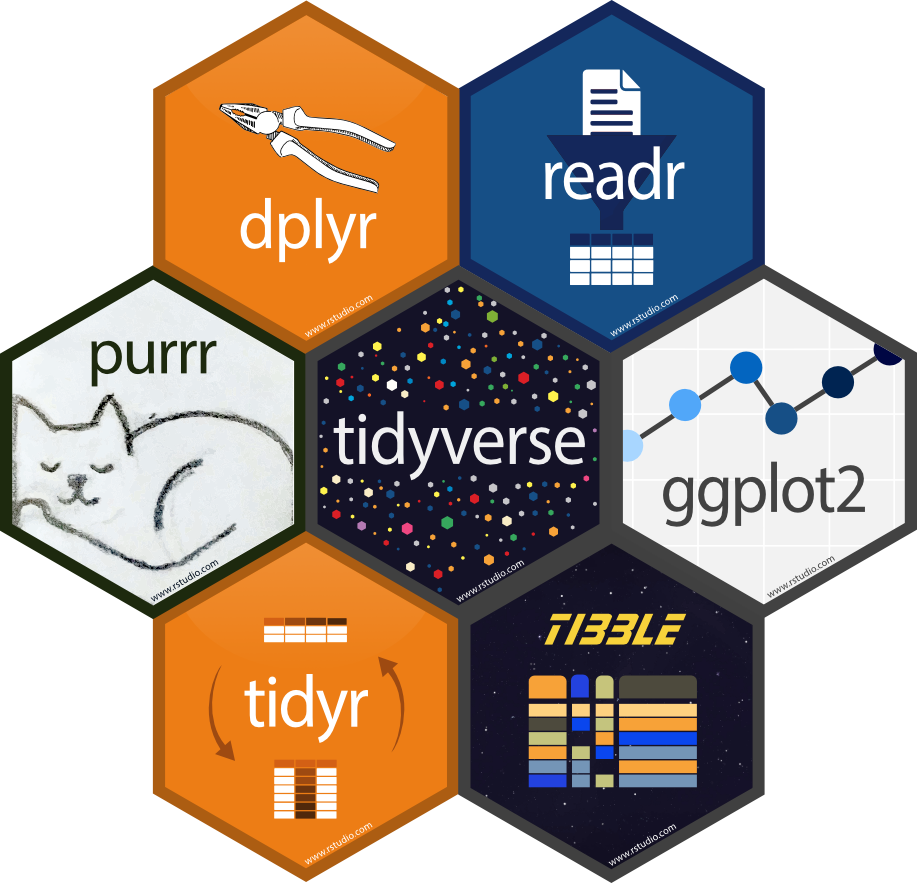
\includegraphics[width=0.4\textwidth,height=0.4\textheight]{Imagenes/tidyverse2.png}

\begin{block}{Paquetes \textbar{} tidyverse}
\protect\hypertarget{paquetes-tidyverse}{}
Principales paquetes incluidos en \texttt{tidyverse}:

\begin{enumerate}
\item
  \textbf{ggplot2}: Para la creación de gráficos y visualizaciones.
\item
  \textbf{dplyr}: Para manipulación y transformación de datos.
\item
  \textbf{tidyr}: Para trabajar con datos en formato ``tidy'' (ordenados
  y estructurados).
\item
  \textbf{readr}: Para la importación limpia y eficiente de datos.
\item
  \textbf{purrr}: Para trabajar con funciones y listas de manera más
  eficiente.
\item
  \textbf{tibble}: Para crear y trabajar con data frames mejorados.
\end{enumerate}
\end{block}

\begin{block}{Beneficios de usar \texttt{tidyverse}:}
\protect\hypertarget{beneficios-de-usar-tidyverse}{}
\begin{enumerate}
\item
  \textbf{Sintaxis coherente}: Los paquetes en \texttt{tidyverse}
  comparten una sintaxis coherente, lo que facilita aprender y recordar
  cómo realizar tareas comunes.
\item
  \textbf{Flujo de trabajo eficiente}: \texttt{tidyverse} está diseñado
  para proporcionar un flujo de trabajo eficiente y fácil de entender,
  desde la importación de datos hasta la visualización de resultados.
\item
  \textbf{Compatibilidad con piped operations}: La tubería
  \texttt{\%\textgreater{}\%} (pipe) facilita la aplicación de
  operaciones en secuencia, lo que mejora la legibilidad del código.
\end{enumerate}
\end{block}

\begin{block}{\texttt{tidyverse}:}
\protect\hypertarget{tidyverse-1}{}
\begin{Shaded}
\begin{Highlighting}[]
\CommentTok{\# Instalar y cargar tidyverse}
\CommentTok{\#install.packages("tidyverse")}
\FunctionTok{library}\NormalTok{(tidyverse)}

\CommentTok{\# Crear un data frame de ejemplo}
\NormalTok{data }\OtherTok{\textless{}{-}} \FunctionTok{data.frame}\NormalTok{(}
  \AttributeTok{ID =} \FunctionTok{c}\NormalTok{(}\DecValTok{1}\NormalTok{, }\DecValTok{2}\NormalTok{, }\DecValTok{3}\NormalTok{, }\DecValTok{4}\NormalTok{, }\DecValTok{5}\NormalTok{),}
  \AttributeTok{Nombre =} \FunctionTok{c}\NormalTok{(}\StringTok{"Juan"}\NormalTok{, }\StringTok{"María"}\NormalTok{, }\StringTok{"Carlos"}\NormalTok{, }\StringTok{"Ana"}\NormalTok{, }\StringTok{"Pedro"}\NormalTok{),}
  \AttributeTok{Edad =} \FunctionTok{c}\NormalTok{(}\DecValTok{25}\NormalTok{, }\DecValTok{30}\NormalTok{, }\DecValTok{22}\NormalTok{, }\DecValTok{28}\NormalTok{, }\DecValTok{35}\NormalTok{)}
\NormalTok{)}
\end{Highlighting}
\end{Shaded}
\end{block}

\begin{block}{\texttt{tidyverse}:}
\protect\hypertarget{tidyverse-2}{}
\begin{Shaded}
\begin{Highlighting}[]
\CommentTok{\# Filtrar personas mayores de 25 años y seleccionar solo las columnas de ID y Nombre}
\NormalTok{resultado }\OtherTok{\textless{}{-}}\NormalTok{ data }\SpecialCharTok{\%\textgreater{}\%}
  \FunctionTok{filter}\NormalTok{(Edad }\SpecialCharTok{\textgreater{}} \DecValTok{25}\NormalTok{) }\SpecialCharTok{\%\textgreater{}\%}
  \FunctionTok{select}\NormalTok{(ID, Nombre)}

\CommentTok{\# Imprimir el resultado}
\FunctionTok{print}\NormalTok{(resultado)}
\end{Highlighting}
\end{Shaded}

\begin{verbatim}
##   ID Nombre
## 1  2  María
## 2  4    Ana
## 3  5  Pedro
\end{verbatim}

\begin{Shaded}
\begin{Highlighting}[]
\CommentTok{\#https://rpubs.com/paraneda/tidyverse}
\end{Highlighting}
\end{Shaded}
\end{block}
\end{frame}

\begin{frame}[fragile]{Practica}
\protect\hypertarget{practica}{}
\begin{block}{Leer Datos}
\protect\hypertarget{leer-datos}{}
\begin{Shaded}
\begin{Highlighting}[]
\DocumentationTok{\#\# La separación decimal en R es . y no ,}
\CommentTok{\#Datos en Millones de Guaranies}
\NormalTok{Ingreso }\OtherTok{\textless{}{-}} \FunctionTok{read.csv}\NormalTok{(}\StringTok{"Datos/IngresoPromPoblacion\_py.csv"}\NormalTok{)}
\NormalTok{Ingreso }\OtherTok{\textless{}{-}} \FunctionTok{read.table}\NormalTok{(}\StringTok{"Datos/IngresoPromPoblacion\_py.csv"}\NormalTok{, }\AttributeTok{header=}\NormalTok{T,}
                    \AttributeTok{na.strings =} \StringTok{"4/"}\NormalTok{, }\AttributeTok{sep=} \StringTok{";"}\NormalTok{, }\AttributeTok{check.names =} \ConstantTok{FALSE}\NormalTok{)}

\NormalTok{Ingreso}
\end{Highlighting}
\end{Shaded}

\begin{verbatim}
##     Departamento  1998  1999  2001  2002  2003  2004  2005  2006  2007  2008
## 1  Alto Paraguay    NA    NA    NA    NA    NA    NA    NA    NA    NA    NA
## 2    Alto Parana 3.467 2.716 2.829 2.345 2.392 2.512 2.511 2.136 2.649 2.760
## 3        Amambay    NA    NA    NA    NA 1.545 1.633    NA    NA    NA    NA
## 4       Asuncion 3.964 3.772 3.660 2.978 3.248 3.251 2.978 3.171 2.943 2.749
## 5       Boqueron    NA    NA    NA    NA    NA    NA    NA    NA    NA    NA
## 6       Caaguazu 1.398 1.488 1.484 1.480 1.734 1.444 1.325 1.336 1.355 1.545
## 7        Caazapa    NA    NA    NA    NA 1.334 1.195    NA    NA    NA    NA
## 8      Canindeyu    NA    NA    NA    NA 2.013 1.871    NA    NA    NA    NA
## 9        Central 2.886 2.624 2.385 1.905 1.959 1.879 2.003 1.956 1.934 2.073
## 10    Concepcion    NA    NA    NA    NA 1.504 1.619    NA    NA    NA    NA
## 11    Cordillera    NA    NA    NA    NA 1.317 1.074    NA    NA    NA    NA
## 12        Guaira    NA    NA    NA    NA 1.209 1.309    NA    NA    NA    NA
## 13        Itapua 2.071 2.277 1.576 1.356 1.868 2.141 1.726 1.477 1.403 2.050
## 14      Misiones    NA    NA    NA    NA 1.394 1.039    NA    NA    NA    NA
## 15      Neembucu    NA    NA    NA    NA 1.006 1.006    NA    NA    NA    NA
## 16     Paraguari    NA    NA    NA    NA 1.150 1.150    NA    NA    NA    NA
## 17    Pte. Hayes    NA    NA    NA    NA    NA    NA    NA    NA    NA    NA
## 18     San Pedro 1.056 1.114 1.230 1.244 1.290 1.260 1.537 1.342 1.447 1.534
##     2009  2010  2011  2012  2013  2014  2015  2016  2017  2018
## 1     NA    NA    NA    NA    NA    NA 2.190 2.317 1.950    NA
## 2  2.332 2.734 2.863 2.476 2.572 2.887 2.813 2.622 2.664 2.663
## 3     NA    NA    NA    NA    NA    NA 2.232 2.580 2.422    NA
## 4  2.688 3.115 3.385 3.274 3.890 4.241 4.300 3.889 4.343 3.529
## 5     NA    NA    NA    NA    NA    NA 5.159 4.443 4.060    NA
## 6  1.786 1.658 1.438 1.553 1.934 2.727 1.706 1.762 2.479 1.921
## 7     NA    NA    NA    NA    NA    NA 2.056 1.555 1.407 1.494
## 8     NA    NA    NA    NA    NA    NA 1.912 2.624 2.206    NA
## 9  2.048 2.152 2.583 2.450 2.705 2.746 2.854 2.591 2.441 2.697
## 10    NA    NA    NA    NA    NA    NA 1.788 1.763 1.518    NA
## 11    NA    NA    NA    NA    NA    NA 1.872 1.780 1.609    NA
## 12    NA    NA    NA    NA    NA    NA 1.715 1.385 1.504    NA
## 13 1.676 1.845 2.350 1.770 1.816 1.891 2.020 1.976 2.073 2.175
## 14    NA    NA    NA    NA    NA    NA 1.862 1.928 1.938    NA
## 15    NA    NA    NA    NA    NA    NA 1.613 1.617 1.806    NA
## 16    NA    NA    NA    NA    NA    NA 1.772 1.515 1.531    NA
## 17    NA    NA    NA    NA    NA    NA 2.586 2.838 2.271    NA
## 18 1.352 1.445 1.572 1.599 2.046 1.898 1.474 1.600 1.818 2.478
\end{verbatim}
\end{block}

\begin{block}{Examinar Datos}
\protect\hypertarget{examinar-datos}{}
\begin{Shaded}
\begin{Highlighting}[]
\DocumentationTok{\#\#Revisar Datos}
\FunctionTok{head}\NormalTok{(Ingreso) }\CommentTok{\#Primeros datos}
\FunctionTok{tail}\NormalTok{(Ingreso) }\CommentTok{\#Ultimos Datos}
\FunctionTok{dim}\NormalTok{(Ingreso) }\CommentTok{\#Tamaño }
\FunctionTok{names}\NormalTok{(Ingreso) }\CommentTok{\#Nombre de Columnas}
\FunctionTok{summary}\NormalTok{(Ingreso) }\CommentTok{\#Sumario de Datos }
\end{Highlighting}
\end{Shaded}
\end{block}
\end{frame}

\begin{frame}{¿Que departamento tiene el mayor ingreso promedio?}
\protect\hypertarget{que-departamento-tiene-el-mayor-ingreso-promedio}{}
\end{frame}

\begin{frame}[fragile]{¿Que departamento tiene el mayor ingreso
promedio?}
\protect\hypertarget{que-departamento-tiene-el-mayor-ingreso-promedio-1}{}
\begin{Shaded}
\begin{Highlighting}[]
\CommentTok{\#Cambiar a datos largos}
\NormalTok{dato\_largo }\OtherTok{\textless{}{-}}\NormalTok{ Ingreso }\SpecialCharTok{\%\textgreater{}\%}
  \FunctionTok{gather}\NormalTok{(}\AttributeTok{key =} \StringTok{"year"}\NormalTok{, }\AttributeTok{value =} \StringTok{"Cantidad"}\NormalTok{, }\SpecialCharTok{{-}}\NormalTok{Departamento) }\SpecialCharTok{\%\textgreater{}\%}
  \FunctionTok{mutate}\NormalTok{(}\AttributeTok{year =} \FunctionTok{as.integer}\NormalTok{(year))}

\NormalTok{dato\_largo}
\end{Highlighting}
\end{Shaded}

\begin{verbatim}
##      Departamento year Cantidad
## 1   Alto Paraguay 1998       NA
## 2     Alto Parana 1998    3.467
## 3         Amambay 1998       NA
## 4        Asuncion 1998    3.964
## 5        Boqueron 1998       NA
## 6        Caaguazu 1998    1.398
## 7         Caazapa 1998       NA
## 8       Canindeyu 1998       NA
## 9         Central 1998    2.886
## 10     Concepcion 1998       NA
## 11     Cordillera 1998       NA
## 12         Guaira 1998       NA
## 13         Itapua 1998    2.071
## 14       Misiones 1998       NA
## 15       Neembucu 1998       NA
## 16      Paraguari 1998       NA
## 17     Pte. Hayes 1998       NA
## 18      San Pedro 1998    1.056
## 19  Alto Paraguay 1999       NA
## 20    Alto Parana 1999    2.716
## 21        Amambay 1999       NA
## 22       Asuncion 1999    3.772
## 23       Boqueron 1999       NA
## 24       Caaguazu 1999    1.488
## 25        Caazapa 1999       NA
## 26      Canindeyu 1999       NA
## 27        Central 1999    2.624
## 28     Concepcion 1999       NA
## 29     Cordillera 1999       NA
## 30         Guaira 1999       NA
## 31         Itapua 1999    2.277
## 32       Misiones 1999       NA
## 33       Neembucu 1999       NA
## 34      Paraguari 1999       NA
## 35     Pte. Hayes 1999       NA
## 36      San Pedro 1999    1.114
## 37  Alto Paraguay 2001       NA
## 38    Alto Parana 2001    2.829
## 39        Amambay 2001       NA
## 40       Asuncion 2001    3.660
## 41       Boqueron 2001       NA
## 42       Caaguazu 2001    1.484
## 43        Caazapa 2001       NA
## 44      Canindeyu 2001       NA
## 45        Central 2001    2.385
## 46     Concepcion 2001       NA
## 47     Cordillera 2001       NA
## 48         Guaira 2001       NA
## 49         Itapua 2001    1.576
## 50       Misiones 2001       NA
## 51       Neembucu 2001       NA
## 52      Paraguari 2001       NA
## 53     Pte. Hayes 2001       NA
## 54      San Pedro 2001    1.230
## 55  Alto Paraguay 2002       NA
## 56    Alto Parana 2002    2.345
## 57        Amambay 2002       NA
## 58       Asuncion 2002    2.978
## 59       Boqueron 2002       NA
## 60       Caaguazu 2002    1.480
## 61        Caazapa 2002       NA
## 62      Canindeyu 2002       NA
## 63        Central 2002    1.905
## 64     Concepcion 2002       NA
## 65     Cordillera 2002       NA
## 66         Guaira 2002       NA
## 67         Itapua 2002    1.356
## 68       Misiones 2002       NA
## 69       Neembucu 2002       NA
## 70      Paraguari 2002       NA
## 71     Pte. Hayes 2002       NA
## 72      San Pedro 2002    1.244
## 73  Alto Paraguay 2003       NA
## 74    Alto Parana 2003    2.392
## 75        Amambay 2003    1.545
## 76       Asuncion 2003    3.248
## 77       Boqueron 2003       NA
## 78       Caaguazu 2003    1.734
## 79        Caazapa 2003    1.334
## 80      Canindeyu 2003    2.013
## 81        Central 2003    1.959
## 82     Concepcion 2003    1.504
## 83     Cordillera 2003    1.317
## 84         Guaira 2003    1.209
## 85         Itapua 2003    1.868
## 86       Misiones 2003    1.394
## 87       Neembucu 2003    1.006
## 88      Paraguari 2003    1.150
## 89     Pte. Hayes 2003       NA
## 90      San Pedro 2003    1.290
## 91  Alto Paraguay 2004       NA
## 92    Alto Parana 2004    2.512
## 93        Amambay 2004    1.633
## 94       Asuncion 2004    3.251
## 95       Boqueron 2004       NA
## 96       Caaguazu 2004    1.444
## 97        Caazapa 2004    1.195
## 98      Canindeyu 2004    1.871
## 99        Central 2004    1.879
## 100    Concepcion 2004    1.619
## 101    Cordillera 2004    1.074
## 102        Guaira 2004    1.309
## 103        Itapua 2004    2.141
## 104      Misiones 2004    1.039
## 105      Neembucu 2004    1.006
## 106     Paraguari 2004    1.150
## 107    Pte. Hayes 2004       NA
## 108     San Pedro 2004    1.260
## 109 Alto Paraguay 2005       NA
## 110   Alto Parana 2005    2.511
## 111       Amambay 2005       NA
## 112      Asuncion 2005    2.978
## 113      Boqueron 2005       NA
## 114      Caaguazu 2005    1.325
## 115       Caazapa 2005       NA
## 116     Canindeyu 2005       NA
## 117       Central 2005    2.003
## 118    Concepcion 2005       NA
## 119    Cordillera 2005       NA
## 120        Guaira 2005       NA
## 121        Itapua 2005    1.726
## 122      Misiones 2005       NA
## 123      Neembucu 2005       NA
## 124     Paraguari 2005       NA
## 125    Pte. Hayes 2005       NA
## 126     San Pedro 2005    1.537
## 127 Alto Paraguay 2006       NA
## 128   Alto Parana 2006    2.136
## 129       Amambay 2006       NA
## 130      Asuncion 2006    3.171
## 131      Boqueron 2006       NA
## 132      Caaguazu 2006    1.336
## 133       Caazapa 2006       NA
## 134     Canindeyu 2006       NA
## 135       Central 2006    1.956
## 136    Concepcion 2006       NA
## 137    Cordillera 2006       NA
## 138        Guaira 2006       NA
## 139        Itapua 2006    1.477
## 140      Misiones 2006       NA
## 141      Neembucu 2006       NA
## 142     Paraguari 2006       NA
## 143    Pte. Hayes 2006       NA
## 144     San Pedro 2006    1.342
## 145 Alto Paraguay 2007       NA
## 146   Alto Parana 2007    2.649
## 147       Amambay 2007       NA
## 148      Asuncion 2007    2.943
## 149      Boqueron 2007       NA
## 150      Caaguazu 2007    1.355
## 151       Caazapa 2007       NA
## 152     Canindeyu 2007       NA
## 153       Central 2007    1.934
## 154    Concepcion 2007       NA
## 155    Cordillera 2007       NA
## 156        Guaira 2007       NA
## 157        Itapua 2007    1.403
## 158      Misiones 2007       NA
## 159      Neembucu 2007       NA
## 160     Paraguari 2007       NA
## 161    Pte. Hayes 2007       NA
## 162     San Pedro 2007    1.447
## 163 Alto Paraguay 2008       NA
## 164   Alto Parana 2008    2.760
## 165       Amambay 2008       NA
## 166      Asuncion 2008    2.749
## 167      Boqueron 2008       NA
## 168      Caaguazu 2008    1.545
## 169       Caazapa 2008       NA
## 170     Canindeyu 2008       NA
## 171       Central 2008    2.073
## 172    Concepcion 2008       NA
## 173    Cordillera 2008       NA
## 174        Guaira 2008       NA
## 175        Itapua 2008    2.050
## 176      Misiones 2008       NA
## 177      Neembucu 2008       NA
## 178     Paraguari 2008       NA
## 179    Pte. Hayes 2008       NA
## 180     San Pedro 2008    1.534
## 181 Alto Paraguay 2009       NA
## 182   Alto Parana 2009    2.332
## 183       Amambay 2009       NA
## 184      Asuncion 2009    2.688
## 185      Boqueron 2009       NA
## 186      Caaguazu 2009    1.786
## 187       Caazapa 2009       NA
## 188     Canindeyu 2009       NA
## 189       Central 2009    2.048
## 190    Concepcion 2009       NA
## 191    Cordillera 2009       NA
## 192        Guaira 2009       NA
## 193        Itapua 2009    1.676
## 194      Misiones 2009       NA
## 195      Neembucu 2009       NA
## 196     Paraguari 2009       NA
## 197    Pte. Hayes 2009       NA
## 198     San Pedro 2009    1.352
## 199 Alto Paraguay 2010       NA
## 200   Alto Parana 2010    2.734
## 201       Amambay 2010       NA
## 202      Asuncion 2010    3.115
## 203      Boqueron 2010       NA
## 204      Caaguazu 2010    1.658
## 205       Caazapa 2010       NA
## 206     Canindeyu 2010       NA
## 207       Central 2010    2.152
## 208    Concepcion 2010       NA
## 209    Cordillera 2010       NA
## 210        Guaira 2010       NA
## 211        Itapua 2010    1.845
## 212      Misiones 2010       NA
## 213      Neembucu 2010       NA
## 214     Paraguari 2010       NA
## 215    Pte. Hayes 2010       NA
## 216     San Pedro 2010    1.445
## 217 Alto Paraguay 2011       NA
## 218   Alto Parana 2011    2.863
## 219       Amambay 2011       NA
## 220      Asuncion 2011    3.385
## 221      Boqueron 2011       NA
## 222      Caaguazu 2011    1.438
## 223       Caazapa 2011       NA
## 224     Canindeyu 2011       NA
## 225       Central 2011    2.583
## 226    Concepcion 2011       NA
## 227    Cordillera 2011       NA
## 228        Guaira 2011       NA
## 229        Itapua 2011    2.350
## 230      Misiones 2011       NA
## 231      Neembucu 2011       NA
## 232     Paraguari 2011       NA
## 233    Pte. Hayes 2011       NA
## 234     San Pedro 2011    1.572
## 235 Alto Paraguay 2012       NA
## 236   Alto Parana 2012    2.476
## 237       Amambay 2012       NA
## 238      Asuncion 2012    3.274
## 239      Boqueron 2012       NA
## 240      Caaguazu 2012    1.553
## 241       Caazapa 2012       NA
## 242     Canindeyu 2012       NA
## 243       Central 2012    2.450
## 244    Concepcion 2012       NA
## 245    Cordillera 2012       NA
## 246        Guaira 2012       NA
## 247        Itapua 2012    1.770
## 248      Misiones 2012       NA
## 249      Neembucu 2012       NA
## 250     Paraguari 2012       NA
## 251    Pte. Hayes 2012       NA
## 252     San Pedro 2012    1.599
## 253 Alto Paraguay 2013       NA
## 254   Alto Parana 2013    2.572
## 255       Amambay 2013       NA
## 256      Asuncion 2013    3.890
## 257      Boqueron 2013       NA
## 258      Caaguazu 2013    1.934
## 259       Caazapa 2013       NA
## 260     Canindeyu 2013       NA
## 261       Central 2013    2.705
## 262    Concepcion 2013       NA
## 263    Cordillera 2013       NA
## 264        Guaira 2013       NA
## 265        Itapua 2013    1.816
## 266      Misiones 2013       NA
## 267      Neembucu 2013       NA
## 268     Paraguari 2013       NA
## 269    Pte. Hayes 2013       NA
## 270     San Pedro 2013    2.046
## 271 Alto Paraguay 2014       NA
## 272   Alto Parana 2014    2.887
## 273       Amambay 2014       NA
## 274      Asuncion 2014    4.241
## 275      Boqueron 2014       NA
## 276      Caaguazu 2014    2.727
## 277       Caazapa 2014       NA
## 278     Canindeyu 2014       NA
## 279       Central 2014    2.746
## 280    Concepcion 2014       NA
## 281    Cordillera 2014       NA
## 282        Guaira 2014       NA
## 283        Itapua 2014    1.891
## 284      Misiones 2014       NA
## 285      Neembucu 2014       NA
## 286     Paraguari 2014       NA
## 287    Pte. Hayes 2014       NA
## 288     San Pedro 2014    1.898
## 289 Alto Paraguay 2015    2.190
## 290   Alto Parana 2015    2.813
## 291       Amambay 2015    2.232
## 292      Asuncion 2015    4.300
## 293      Boqueron 2015    5.159
## 294      Caaguazu 2015    1.706
## 295       Caazapa 2015    2.056
## 296     Canindeyu 2015    1.912
## 297       Central 2015    2.854
## 298    Concepcion 2015    1.788
## 299    Cordillera 2015    1.872
## 300        Guaira 2015    1.715
## 301        Itapua 2015    2.020
## 302      Misiones 2015    1.862
## 303      Neembucu 2015    1.613
## 304     Paraguari 2015    1.772
## 305    Pte. Hayes 2015    2.586
## 306     San Pedro 2015    1.474
## 307 Alto Paraguay 2016    2.317
## 308   Alto Parana 2016    2.622
## 309       Amambay 2016    2.580
## 310      Asuncion 2016    3.889
## 311      Boqueron 2016    4.443
## 312      Caaguazu 2016    1.762
## 313       Caazapa 2016    1.555
## 314     Canindeyu 2016    2.624
## 315       Central 2016    2.591
## 316    Concepcion 2016    1.763
## 317    Cordillera 2016    1.780
## 318        Guaira 2016    1.385
## 319        Itapua 2016    1.976
## 320      Misiones 2016    1.928
## 321      Neembucu 2016    1.617
## 322     Paraguari 2016    1.515
## 323    Pte. Hayes 2016    2.838
## 324     San Pedro 2016    1.600
## 325 Alto Paraguay 2017    1.950
## 326   Alto Parana 2017    2.664
## 327       Amambay 2017    2.422
## 328      Asuncion 2017    4.343
## 329      Boqueron 2017    4.060
## 330      Caaguazu 2017    2.479
## 331       Caazapa 2017    1.407
## 332     Canindeyu 2017    2.206
## 333       Central 2017    2.441
## 334    Concepcion 2017    1.518
## 335    Cordillera 2017    1.609
## 336        Guaira 2017    1.504
## 337        Itapua 2017    2.073
## 338      Misiones 2017    1.938
## 339      Neembucu 2017    1.806
## 340     Paraguari 2017    1.531
## 341    Pte. Hayes 2017    2.271
## 342     San Pedro 2017    1.818
## 343 Alto Paraguay 2018       NA
## 344   Alto Parana 2018    2.663
## 345       Amambay 2018       NA
## 346      Asuncion 2018    3.529
## 347      Boqueron 2018       NA
## 348      Caaguazu 2018    1.921
## 349       Caazapa 2018    1.494
## 350     Canindeyu 2018       NA
## 351       Central 2018    2.697
## 352    Concepcion 2018       NA
## 353    Cordillera 2018       NA
## 354        Guaira 2018       NA
## 355        Itapua 2018    2.175
## 356      Misiones 2018       NA
## 357      Neembucu 2018       NA
## 358     Paraguari 2018       NA
## 359    Pte. Hayes 2018       NA
## 360     San Pedro 2018    2.478
\end{verbatim}

\begin{block}{¿Que departamento tiene el mayor ingreso promedio?}
\protect\hypertarget{que-departamento-tiene-el-mayor-ingreso-promedio-2}{}
\begin{Shaded}
\begin{Highlighting}[]
\CommentTok{\#Limpiar Datos}
\CommentTok{\# Recortar espacios en blanco en columnas}
\NormalTok{dato\_largo}\SpecialCharTok{$}\NormalTok{Departamento }\OtherTok{\textless{}{-}} \FunctionTok{str\_trim}\NormalTok{(dato\_largo}\SpecialCharTok{$}\NormalTok{Departamento) }

\CommentTok{\# Reemplzar espacios en blanco en columnas}
\NormalTok{dato\_largo}\SpecialCharTok{$}\NormalTok{Departamento }\OtherTok{\textless{}{-}} \FunctionTok{str\_replace}\NormalTok{(dato\_largo}\SpecialCharTok{$}\NormalTok{Departamento, }\StringTok{\textquotesingle{} \textquotesingle{}}\NormalTok{, }\StringTok{\textquotesingle{}\_\textquotesingle{}}\NormalTok{) }

\CommentTok{\# Reemplazar ciertos valores}
\FunctionTok{any}\NormalTok{(}\FunctionTok{is.na}\NormalTok{(dato\_largo))  }\CommentTok{\# Verificar valores faltantes (NAs)}
\end{Highlighting}
\end{Shaded}

\begin{verbatim}
## [1] TRUE
\end{verbatim}

\begin{Shaded}
\begin{Highlighting}[]
\CommentTok{\#dato\_largo[is.na(dato\_largo)] \textless{}{-} 0  \# Reemplazar NAs con 0s}
\end{Highlighting}
\end{Shaded}
\end{block}

\begin{block}{¿Que departamento tiene el mayor ingreso promedio?}
\protect\hypertarget{que-departamento-tiene-el-mayor-ingreso-promedio-3}{}
\begin{Shaded}
\begin{Highlighting}[]
\CommentTok{\# Agrupar los datos por departamento y encontrar el departamento con el mayor ingreso promedio}
\NormalTok{Mayor\_Departamento }\OtherTok{\textless{}{-}}\NormalTok{ dato\_largo }\SpecialCharTok{\%\textgreater{}\%}
  \FunctionTok{group\_by}\NormalTok{(Departamento) }\SpecialCharTok{\%\textgreater{}\%}
  \FunctionTok{summarize}\NormalTok{(}\AttributeTok{Cantidad\_total =} \FunctionTok{mean}\NormalTok{(Cantidad, }\AttributeTok{na.rm =} \ConstantTok{TRUE}\NormalTok{)) }\SpecialCharTok{\%\textgreater{}\%}
  \FunctionTok{slice}\NormalTok{(}\FunctionTok{which.max}\NormalTok{(Cantidad\_total)) }\SpecialCharTok{\%\textgreater{}\%}
  \FunctionTok{ungroup}\NormalTok{()}
\end{Highlighting}
\end{Shaded}
\end{block}

\begin{block}{¿Que departamento tiene el mayor ingreso promedio?}
\protect\hypertarget{que-departamento-tiene-el-mayor-ingreso-promedio-4}{}
\begin{verbatim}
## # A tibble: 1 x 2
##   Departamento Cantidad_total
##   <chr>                 <dbl>
## 1 Boqueron               4.55
\end{verbatim}
\end{block}

\begin{block}{Otras Preguntas}
\protect\hypertarget{otras-preguntas}{}
\begin{Shaded}
\begin{Highlighting}[]
\CommentTok{\#Departamentos con ingresos mayor a 2.5 luego del 2000}
\NormalTok{resultados }\OtherTok{\textless{}{-}}\NormalTok{ dato\_largo }\SpecialCharTok{\%\textgreater{}\%}
  \FunctionTok{filter}\NormalTok{(Cantidad }\SpecialCharTok{\textgreater{}} \FloatTok{2.5} \SpecialCharTok{\&}\NormalTok{ year }\SpecialCharTok{\textgreater{}} \DecValTok{2000}\NormalTok{) }\SpecialCharTok{\%\textgreater{}\%}
  \FunctionTok{select}\NormalTok{(Departamento, year, Cantidad)}

\NormalTok{resultados}
\end{Highlighting}
\end{Shaded}

\begin{verbatim}
##    Departamento year Cantidad
## 1   Alto_Parana 2001    2.829
## 2      Asuncion 2001    3.660
## 3      Asuncion 2002    2.978
## 4      Asuncion 2003    3.248
## 5   Alto_Parana 2004    2.512
## 6      Asuncion 2004    3.251
## 7   Alto_Parana 2005    2.511
## 8      Asuncion 2005    2.978
## 9      Asuncion 2006    3.171
## 10  Alto_Parana 2007    2.649
## 11     Asuncion 2007    2.943
## 12  Alto_Parana 2008    2.760
## 13     Asuncion 2008    2.749
## 14     Asuncion 2009    2.688
## 15  Alto_Parana 2010    2.734
## 16     Asuncion 2010    3.115
## 17  Alto_Parana 2011    2.863
## 18     Asuncion 2011    3.385
## 19      Central 2011    2.583
## 20     Asuncion 2012    3.274
## 21  Alto_Parana 2013    2.572
## 22     Asuncion 2013    3.890
## 23      Central 2013    2.705
## 24  Alto_Parana 2014    2.887
## 25     Asuncion 2014    4.241
## 26     Caaguazu 2014    2.727
## 27      Central 2014    2.746
## 28  Alto_Parana 2015    2.813
## 29     Asuncion 2015    4.300
## 30     Boqueron 2015    5.159
## 31      Central 2015    2.854
## 32   Pte._Hayes 2015    2.586
## 33  Alto_Parana 2016    2.622
## 34      Amambay 2016    2.580
## 35     Asuncion 2016    3.889
## 36     Boqueron 2016    4.443
## 37    Canindeyu 2016    2.624
## 38      Central 2016    2.591
## 39   Pte._Hayes 2016    2.838
## 40  Alto_Parana 2017    2.664
## 41     Asuncion 2017    4.343
## 42     Boqueron 2017    4.060
## 43  Alto_Parana 2018    2.663
## 44     Asuncion 2018    3.529
## 45      Central 2018    2.697
\end{verbatim}
\end{block}

\begin{block}{Graficar}
\protect\hypertarget{graficar}{}
\includegraphics{Intro_aR_2023_presentacion_files/figure-beamer/unnamed-chunk-43-1.pdf}
\end{block}

\begin{block}{Otras Preguntas}
\protect\hypertarget{otras-preguntas-1}{}
\begin{Shaded}
\begin{Highlighting}[]
\CommentTok{\#Seleccionar Solo datos de Itapua}
\NormalTok{dato\_largo\_itapua }\OtherTok{\textless{}{-}}\NormalTok{ dato\_largo[dato\_largo}\SpecialCharTok{$}\NormalTok{Departamento }\SpecialCharTok{==} \StringTok{"Itapua"}\NormalTok{, ]}
\NormalTok{Ingreso\_Promedio\_itapua }\OtherTok{\textless{}{-}}\NormalTok{  dato\_largo\_itapua}\SpecialCharTok{$}\NormalTok{Cantidad}

\CommentTok{\#Seleccionar Solo datos de Itapua}
\NormalTok{dato\_largo\_Boqueron }\OtherTok{\textless{}{-}}\NormalTok{ dato\_largo[dato\_largo}\SpecialCharTok{$}\NormalTok{Departamento }\SpecialCharTok{==} \StringTok{"Boqueron"}\NormalTok{, ]}
\NormalTok{Ingreso\_Promedio\_Boqueron }\OtherTok{\textless{}{-}}\NormalTok{  dato\_largo\_Boqueron}\SpecialCharTok{$}\NormalTok{Cantidad}
\end{Highlighting}
\end{Shaded}
\end{block}
\end{frame}

\end{document}
